\documentclass{article}

\usepackage[utf8]{inputenc}
\usepackage{graphicx}
\usepackage{url}
\usepackage{color}
\usepackage{titlesec}
\usepackage{amsmath}
\usepackage{physics}
\usepackage{amsfonts}
\usepackage{subcaption}
\graphicspath{{../figures/}}

\title{paper draft: supersat}
\author{K. Latimer}
\date{Jan 13, 2020}

\begin{document}

\maketitle


\section{Introduction}
introductory notes.
\section{Theory + Simulation}
\begin{itemize}
	\item brief statement of quasi steady state formula 
	\item we see agreement between actual and QSS supersaturation under the conditions (see fig \ref{wrfvsqss}):
	\begin{itemize}
		\item T \textgreater  273K (we're not including ice in the theory)
		\item w \textgreater  2 m/s (reasonably strong updrafts)
		\item cloud LWC \textgreater  1e-4 g/g (in the convection core)
		\item including rain droplets and ventillation corrections
	\end{itemize}
	\item upon applying above filters, the distributions of $SS_{QSS}$, LWC (cloud only) and $w$, are shown in figs \ref{wrfssqsshist}, \ref{wrfwhist}, and \ref{wrflwchist}.
\end{itemize}
\begin{figure}[ht]
	\centering
	\begin{subfigure}{0.7\textwidth}
		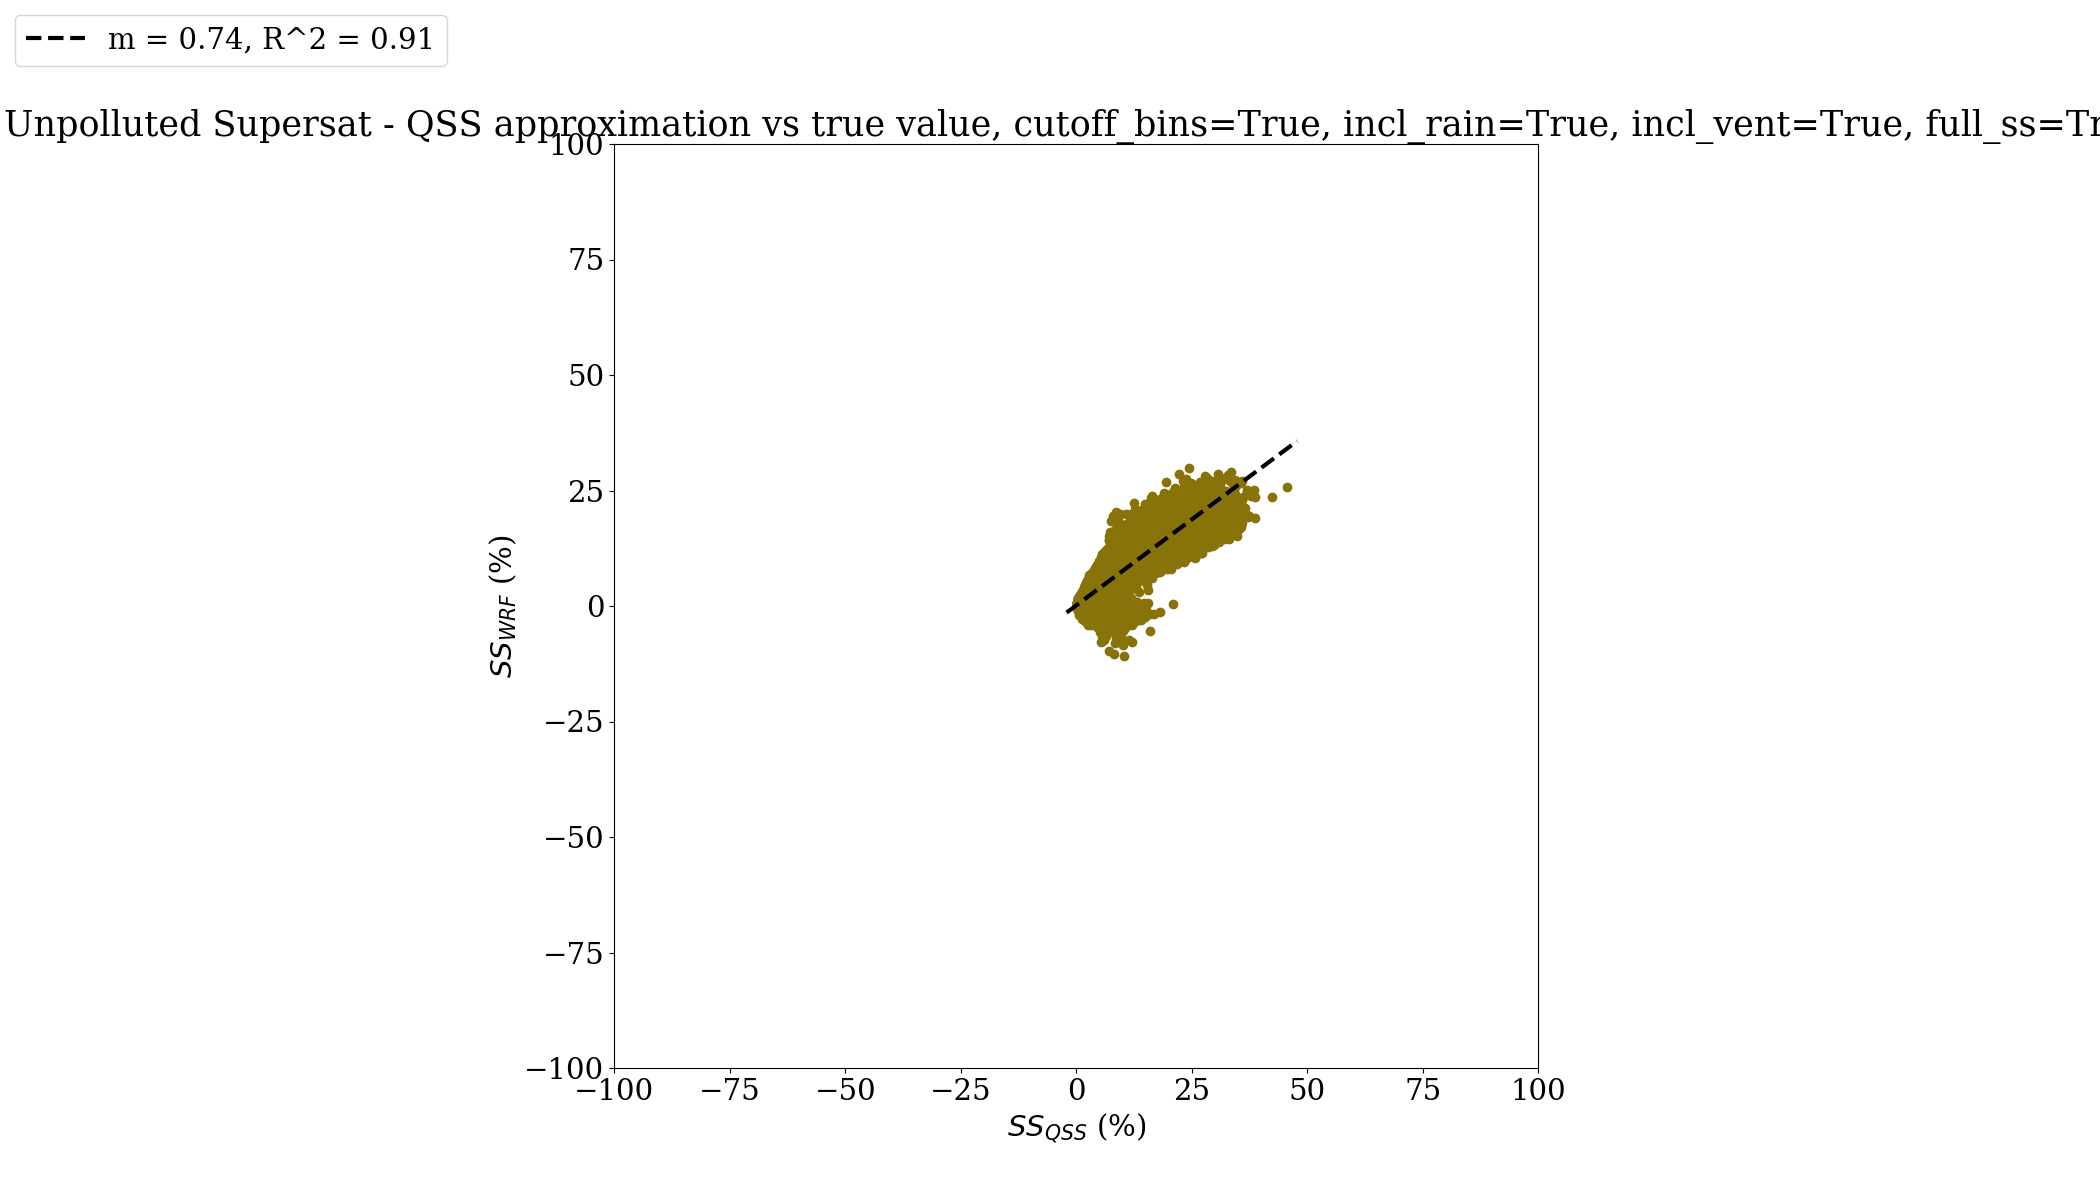
\includegraphics[width=\textwidth]{revmywrf/v12_ss_qss_vs_ss_wrf_Unpolluted_figure.png}
		\caption{Unpolluted case.}
		\label{wrfvsqssunpoll}
	\end{subfigure}
	\begin{subfigure}{0.7\textwidth}
		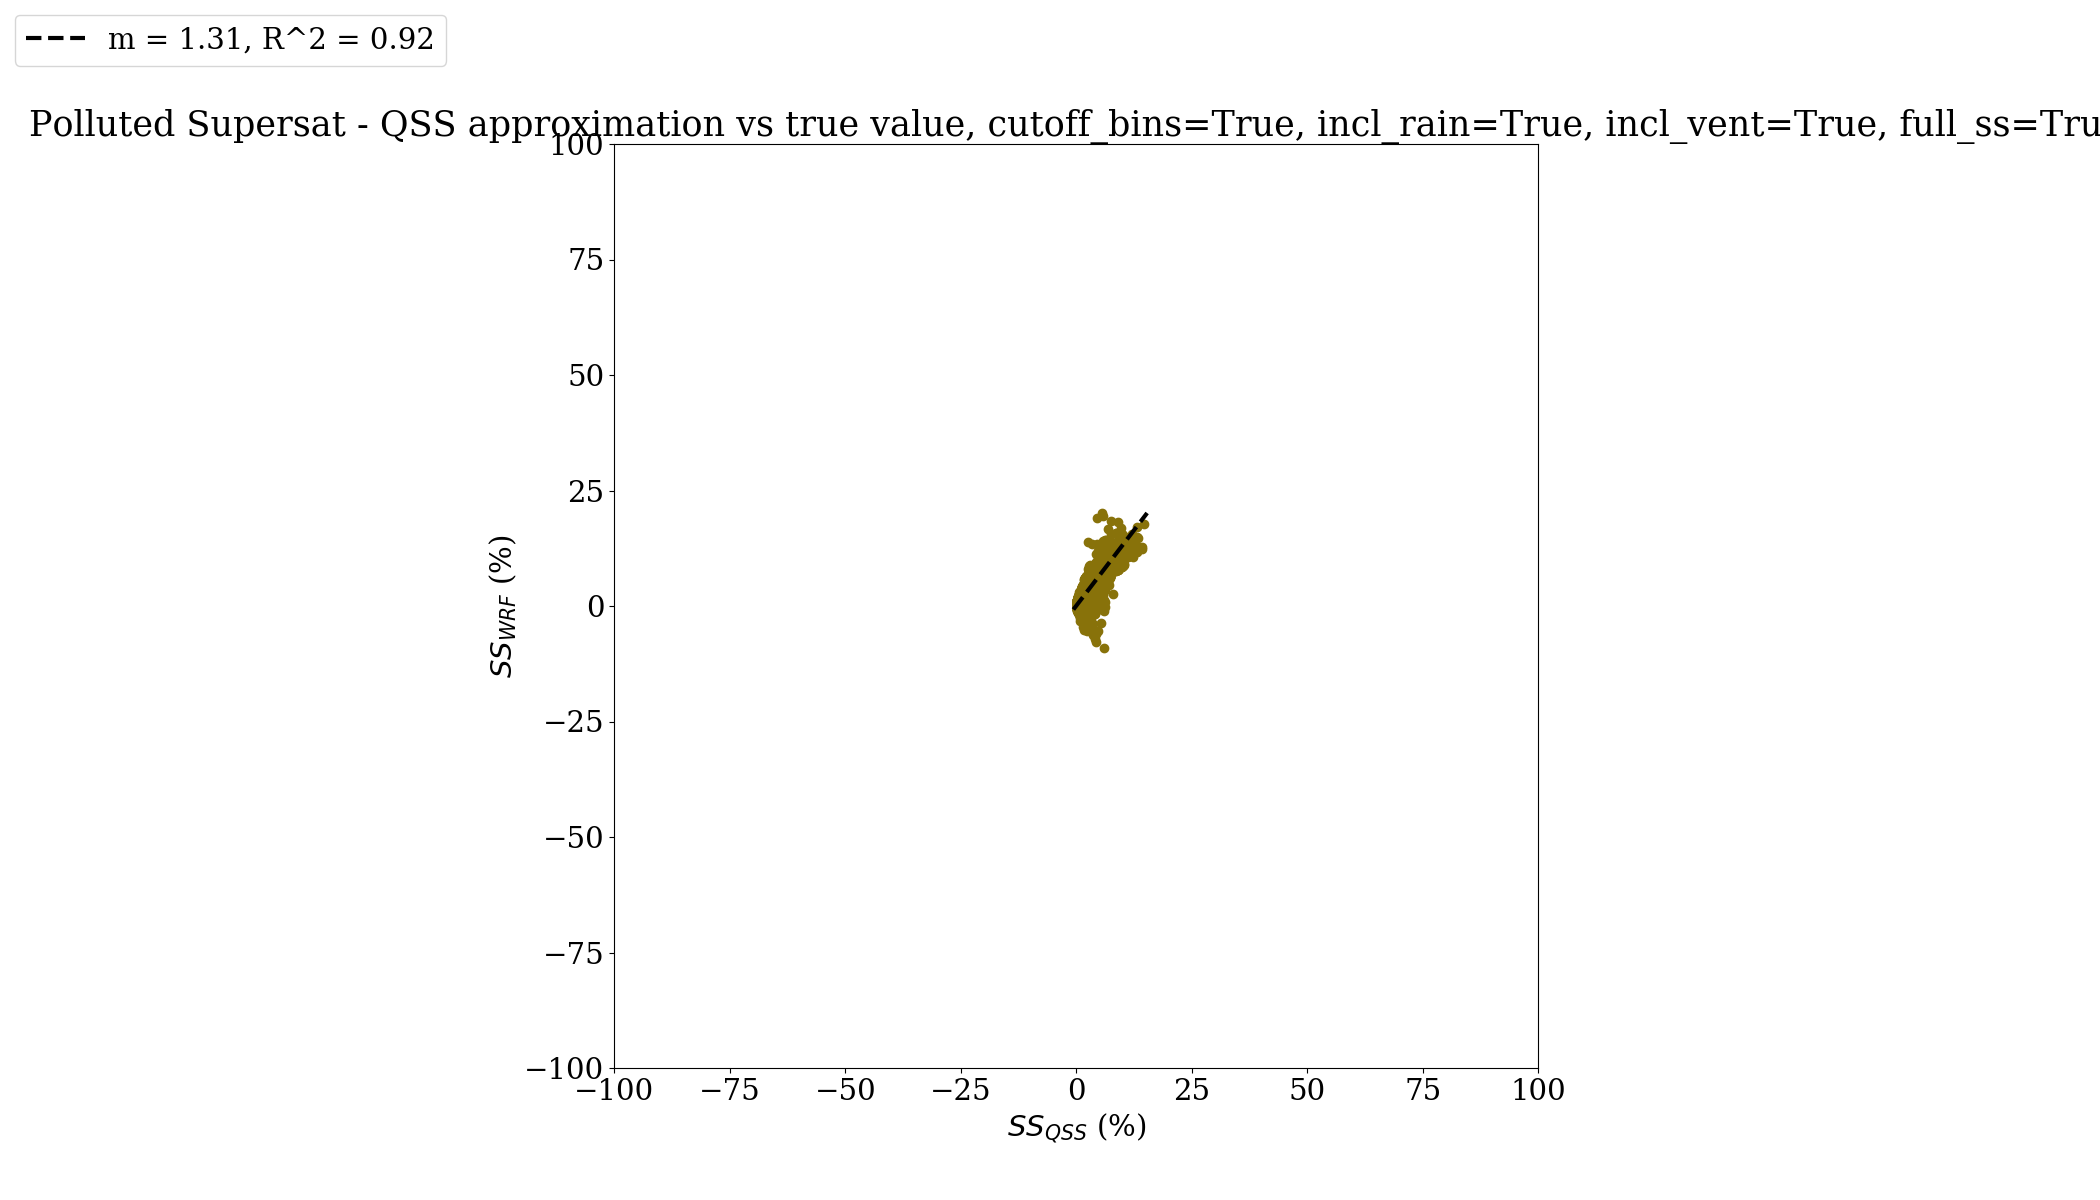
\includegraphics[width=\textwidth]{revmywrf/v12_ss_qss_vs_ss_wrf_Polluted_figure.png}
		\caption{Polluted case.}
		\label{wrfvsqsspoll}
	\end{subfigure}
	\caption{Actual ($SS_{WRF}$) vs predicted ($SS_{QSS}$) supersaturation.}
	\label{wrfvsqss}
\end{figure}
\begin{figure}[ht]
	\centering
	\begin{subfigure}{0.7\textwidth}
		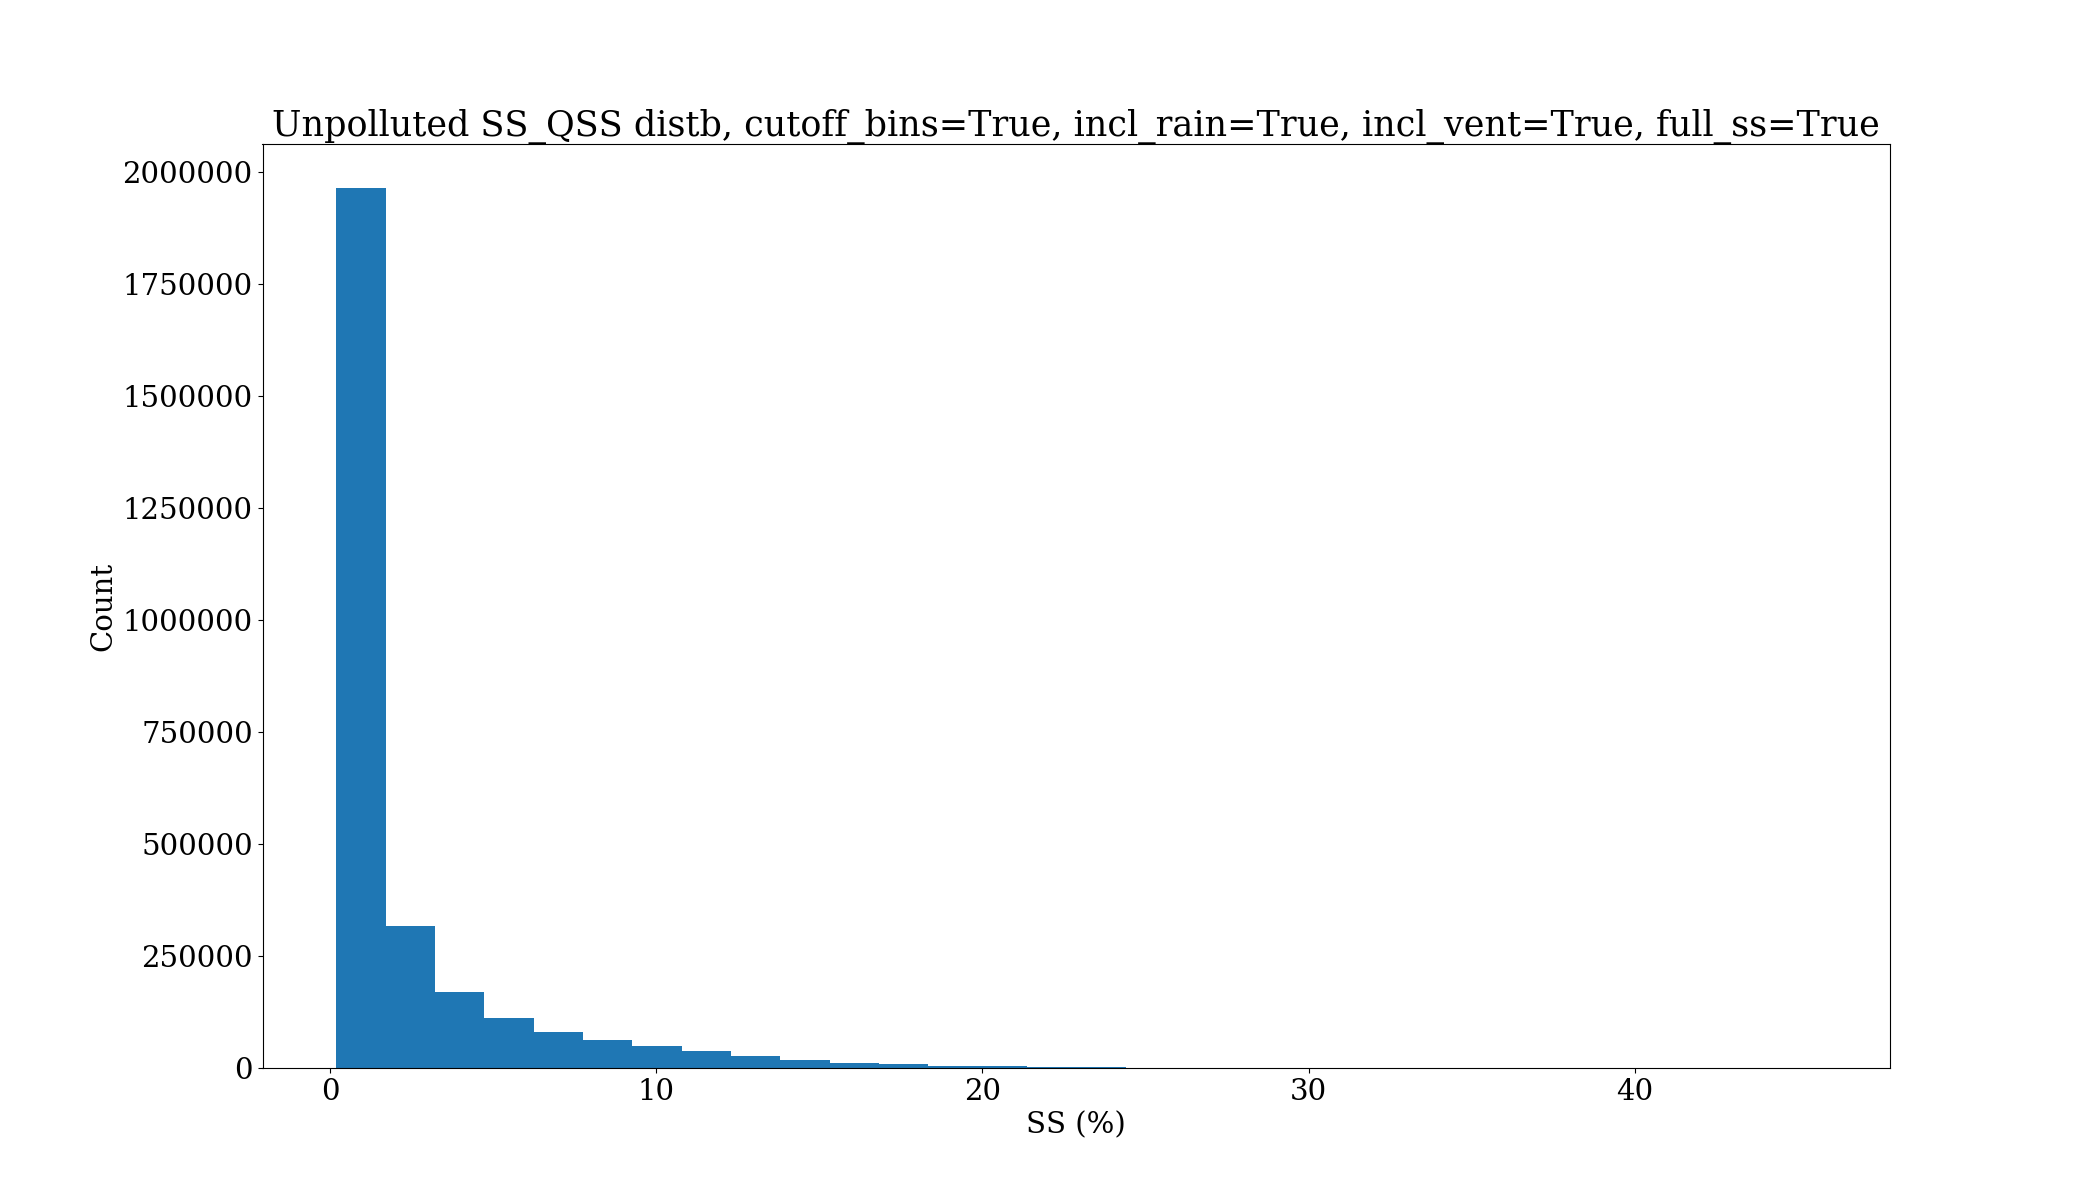
\includegraphics[width=\textwidth]{revmywrf/v12_ss_qss_hist_Unpolluted_figure.png}
		\caption{Unpolluted case.}
		\label{wrfssqsshistunpoll}
	\end{subfigure}
	\begin{subfigure}{0.7\textwidth}
		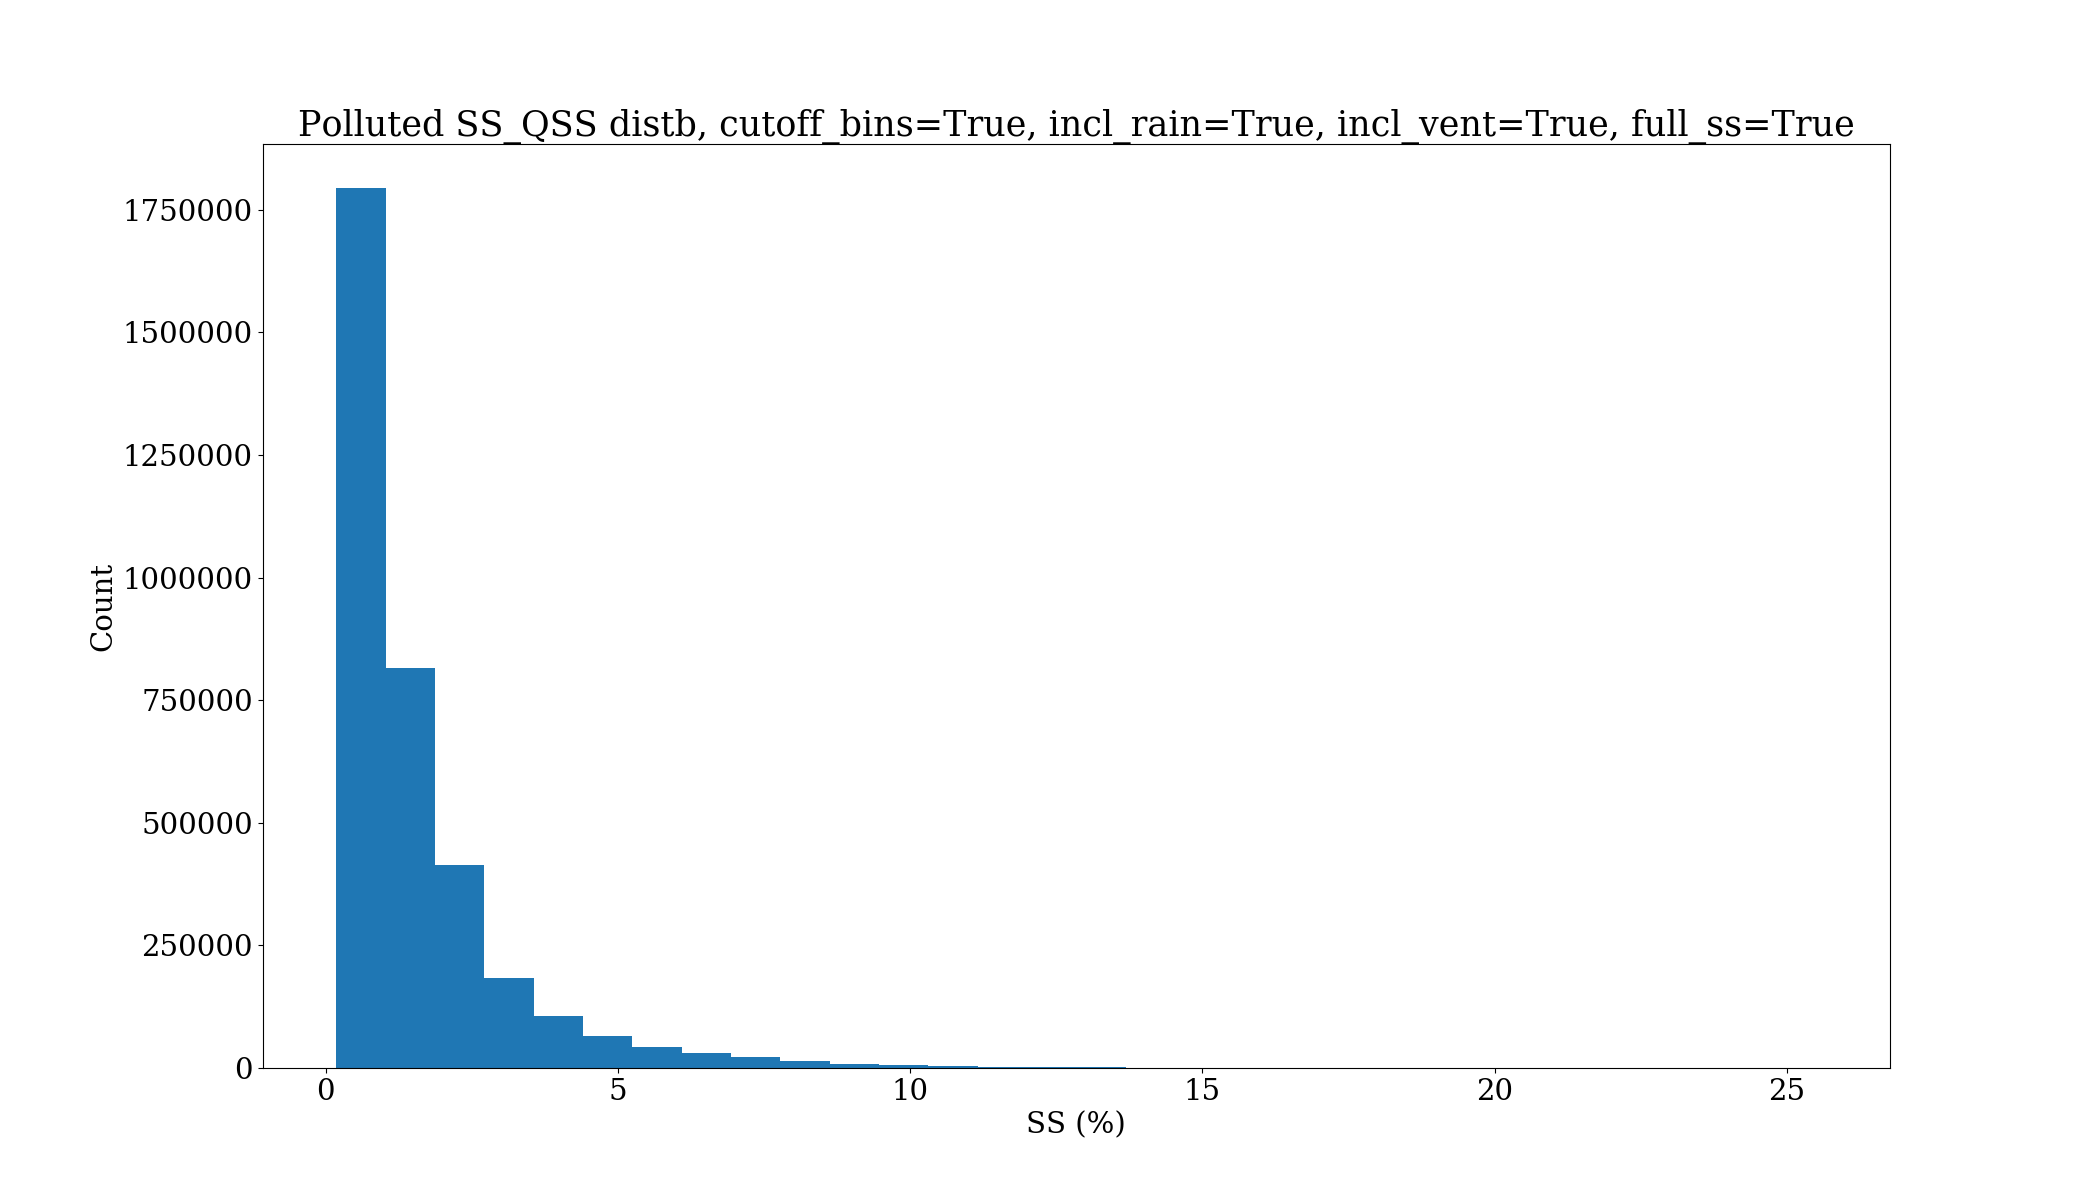
\includegraphics[width=\textwidth]{revmywrf/v12_ss_qss_hist_Polluted_figure.png}
		\caption{Polluted case.}
		\label{wrfssqsshistpoll}
	\end{subfigure}
	\caption{$SS_{WRF}$ distribution in WRF simulation using filtering criteria described in the text.}
	\label{wrfssqsshist}
\end{figure}
\begin{figure}[ht]
	\centering
	\begin{subfigure}{0.7\textwidth}
		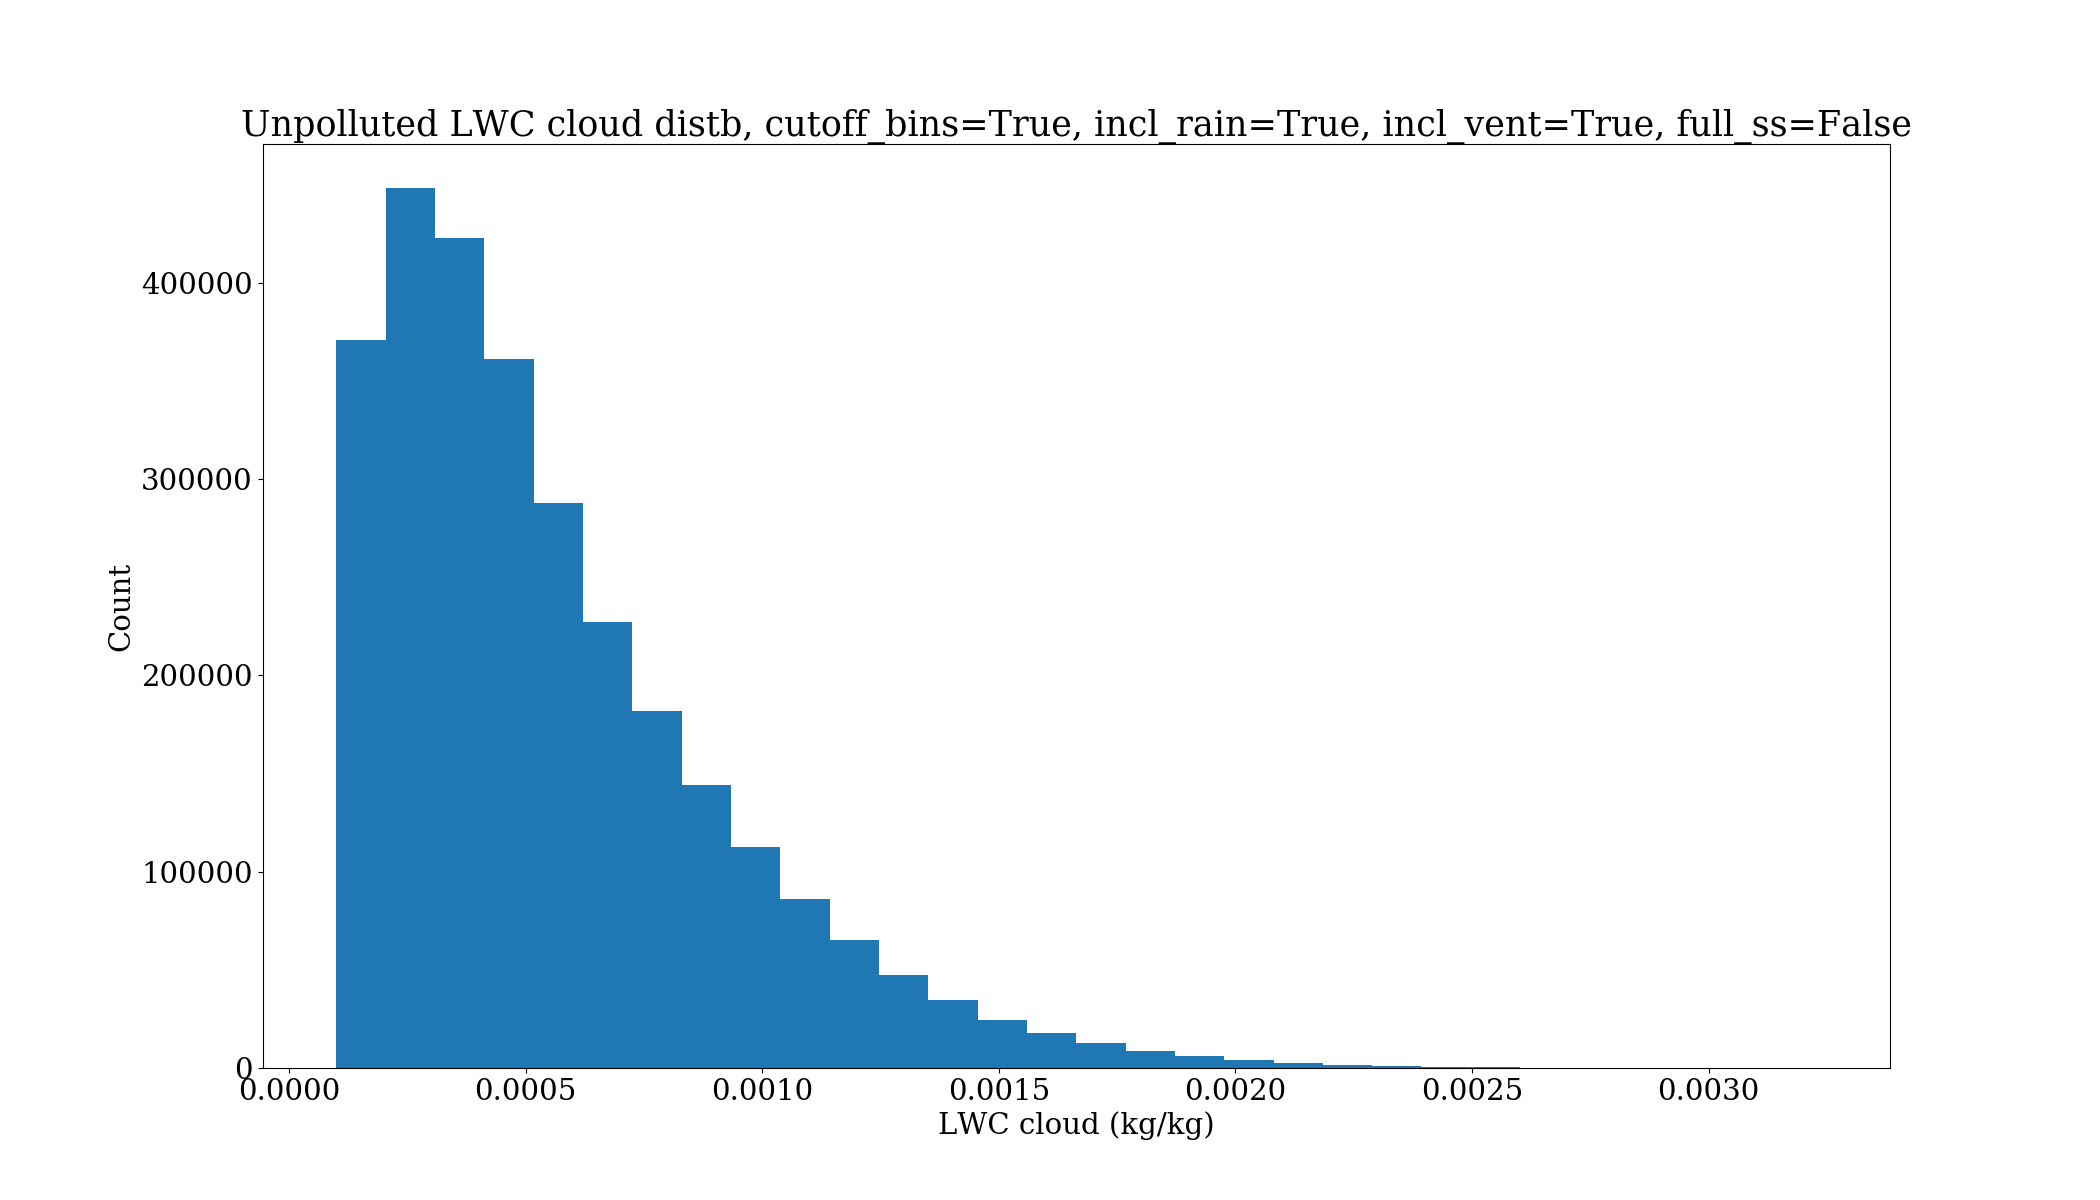
\includegraphics[width=\textwidth]{revmywrf/v9_lwc_hist_Unpolluted_figure.png}
		\caption{Unpolluted case.}
		\label{wrflwchistunpoll}
	\end{subfigure}
	\begin{subfigure}{0.7\textwidth}
		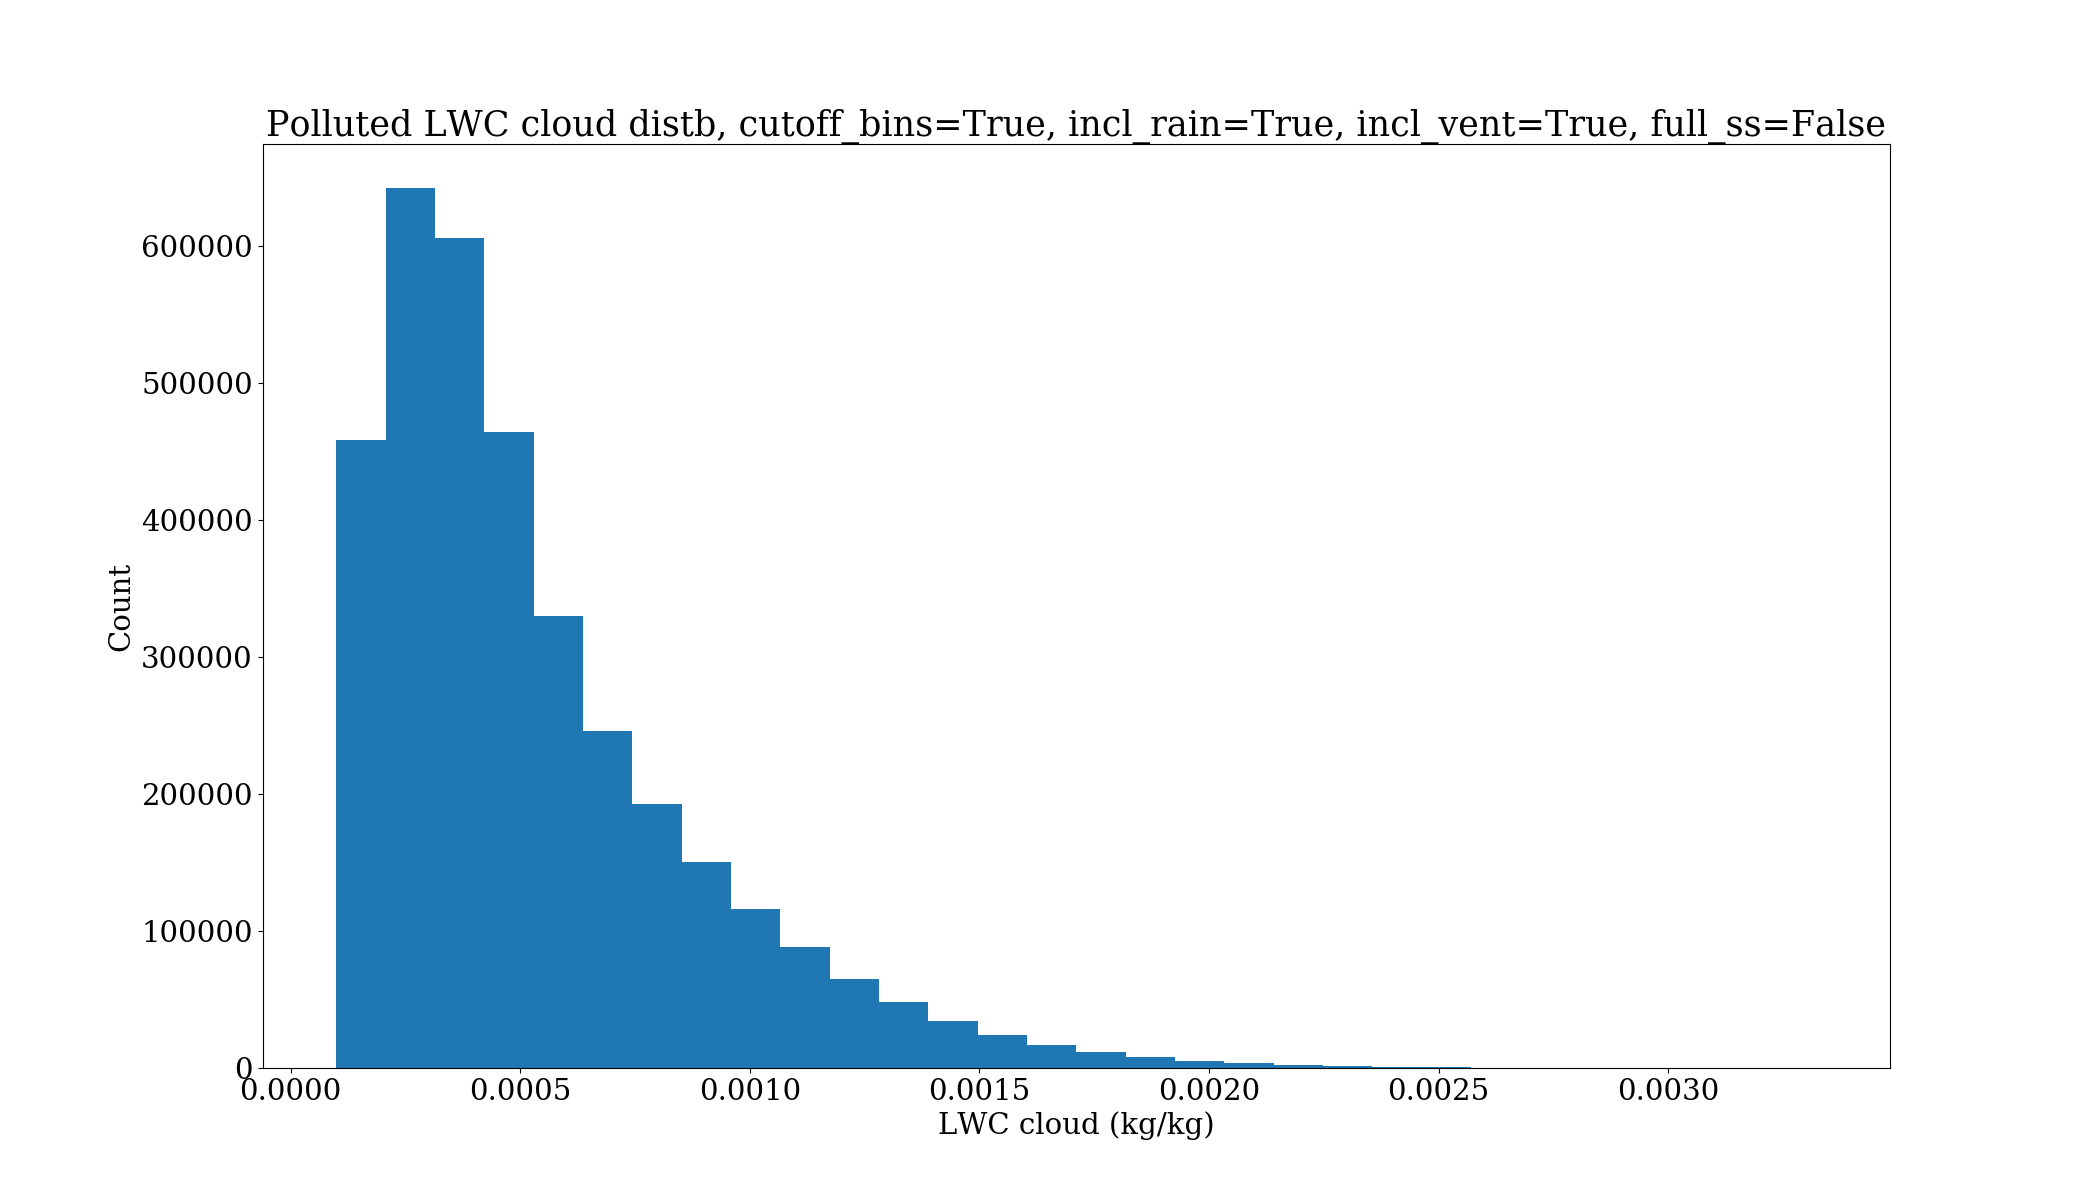
\includegraphics[width=\textwidth]{revmywrf/v9_lwc_hist_Polluted_figure.png}
		\caption{Polluted case.}
		\label{wrflwchistpoll}
	\end{subfigure}
	\caption{Cloud LWC distribution in WRF simulation using filtering criteria described in the text.}
	\label{wrflwchist}
\end{figure}
\begin{figure}[ht]
	\centering
	\begin{subfigure}{0.7\textwidth}
		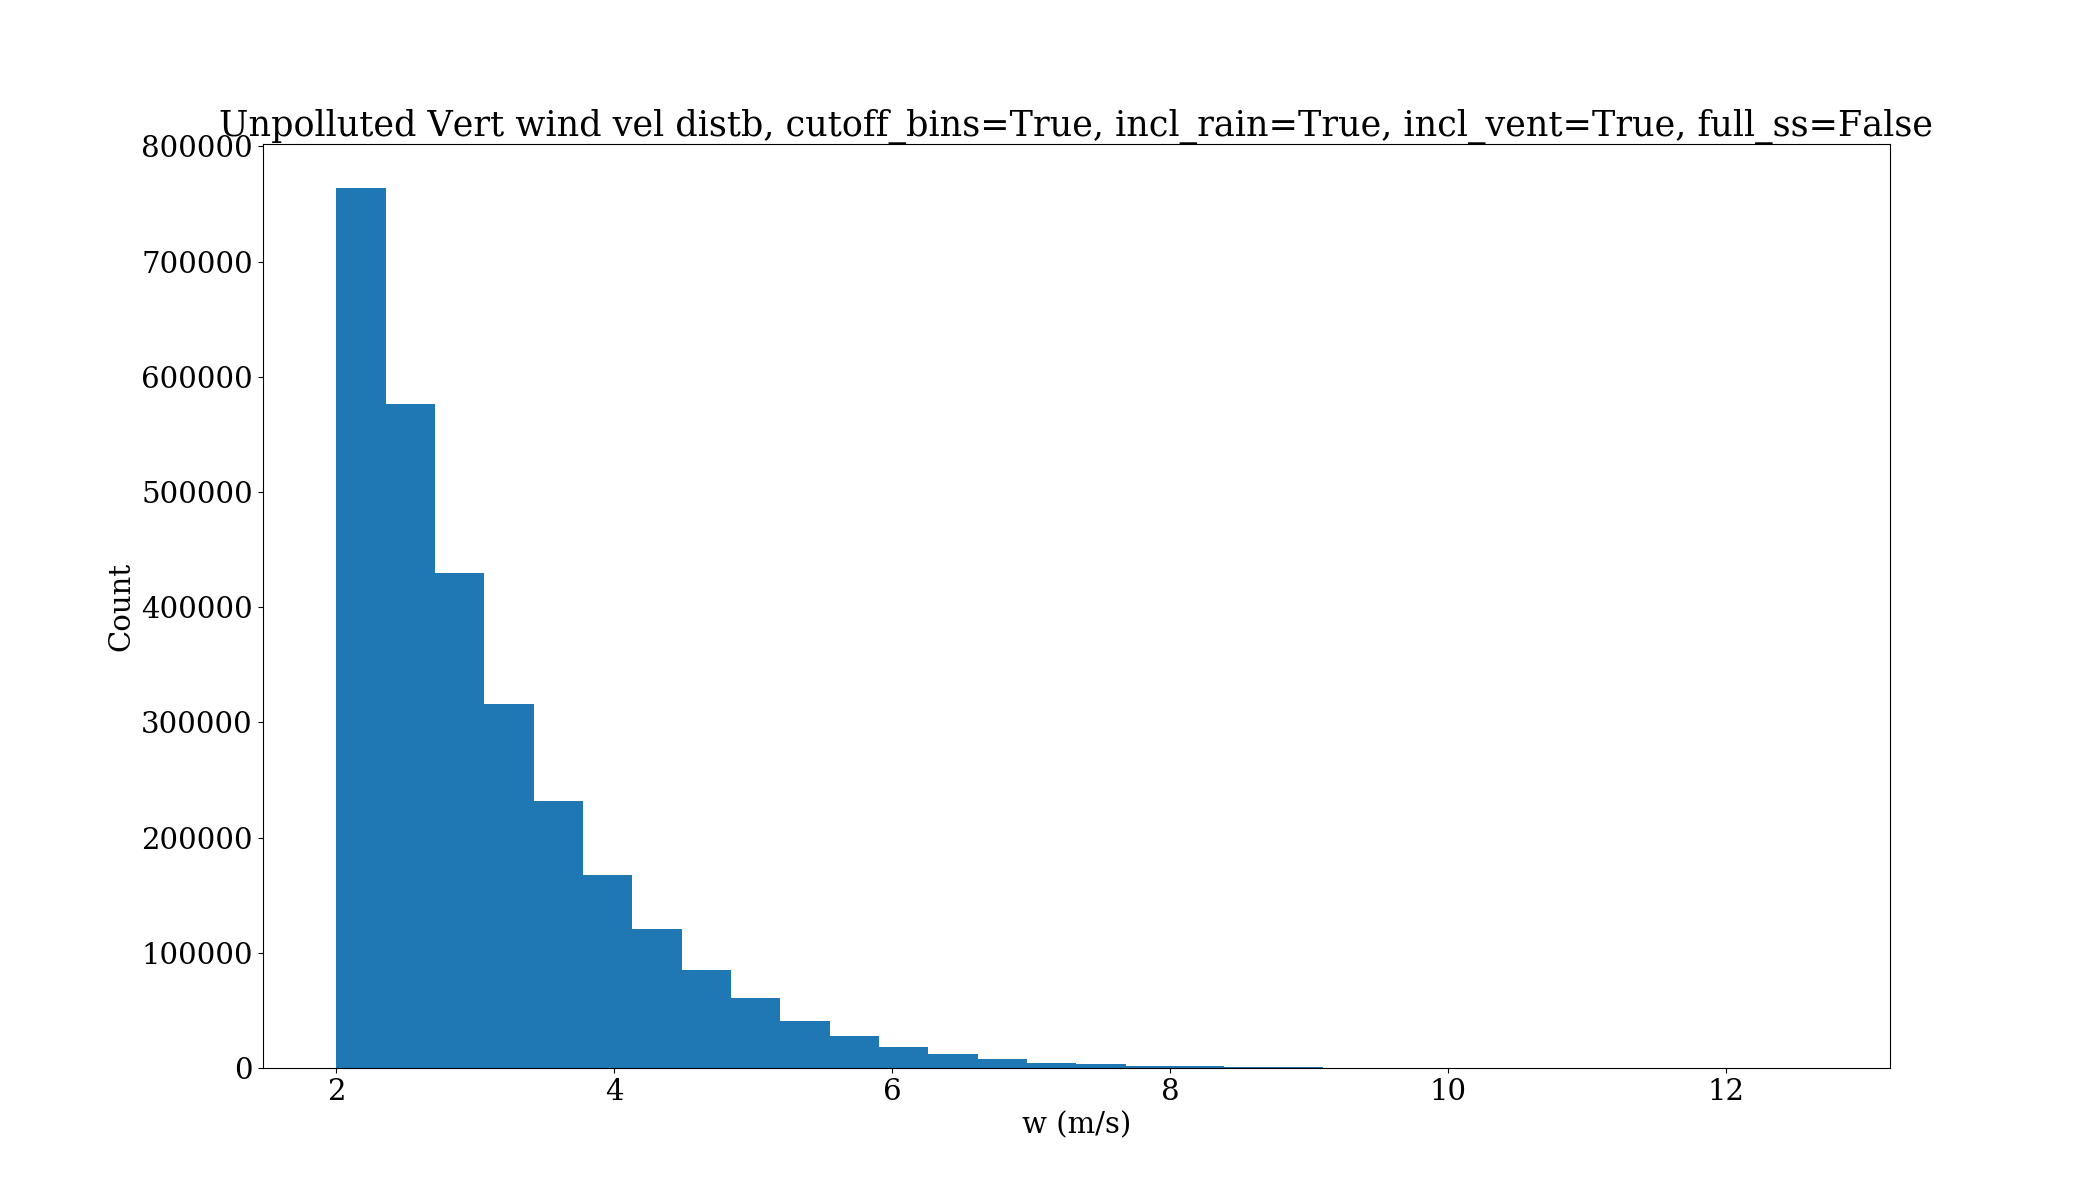
\includegraphics[width=\textwidth]{revmywrf/v9_w_hist_Unpolluted_figure.png}
		\caption{Unpolluted case.}
		\label{wrfwhistunpoll}
	\end{subfigure}
	\begin{subfigure}{0.7\textwidth}
		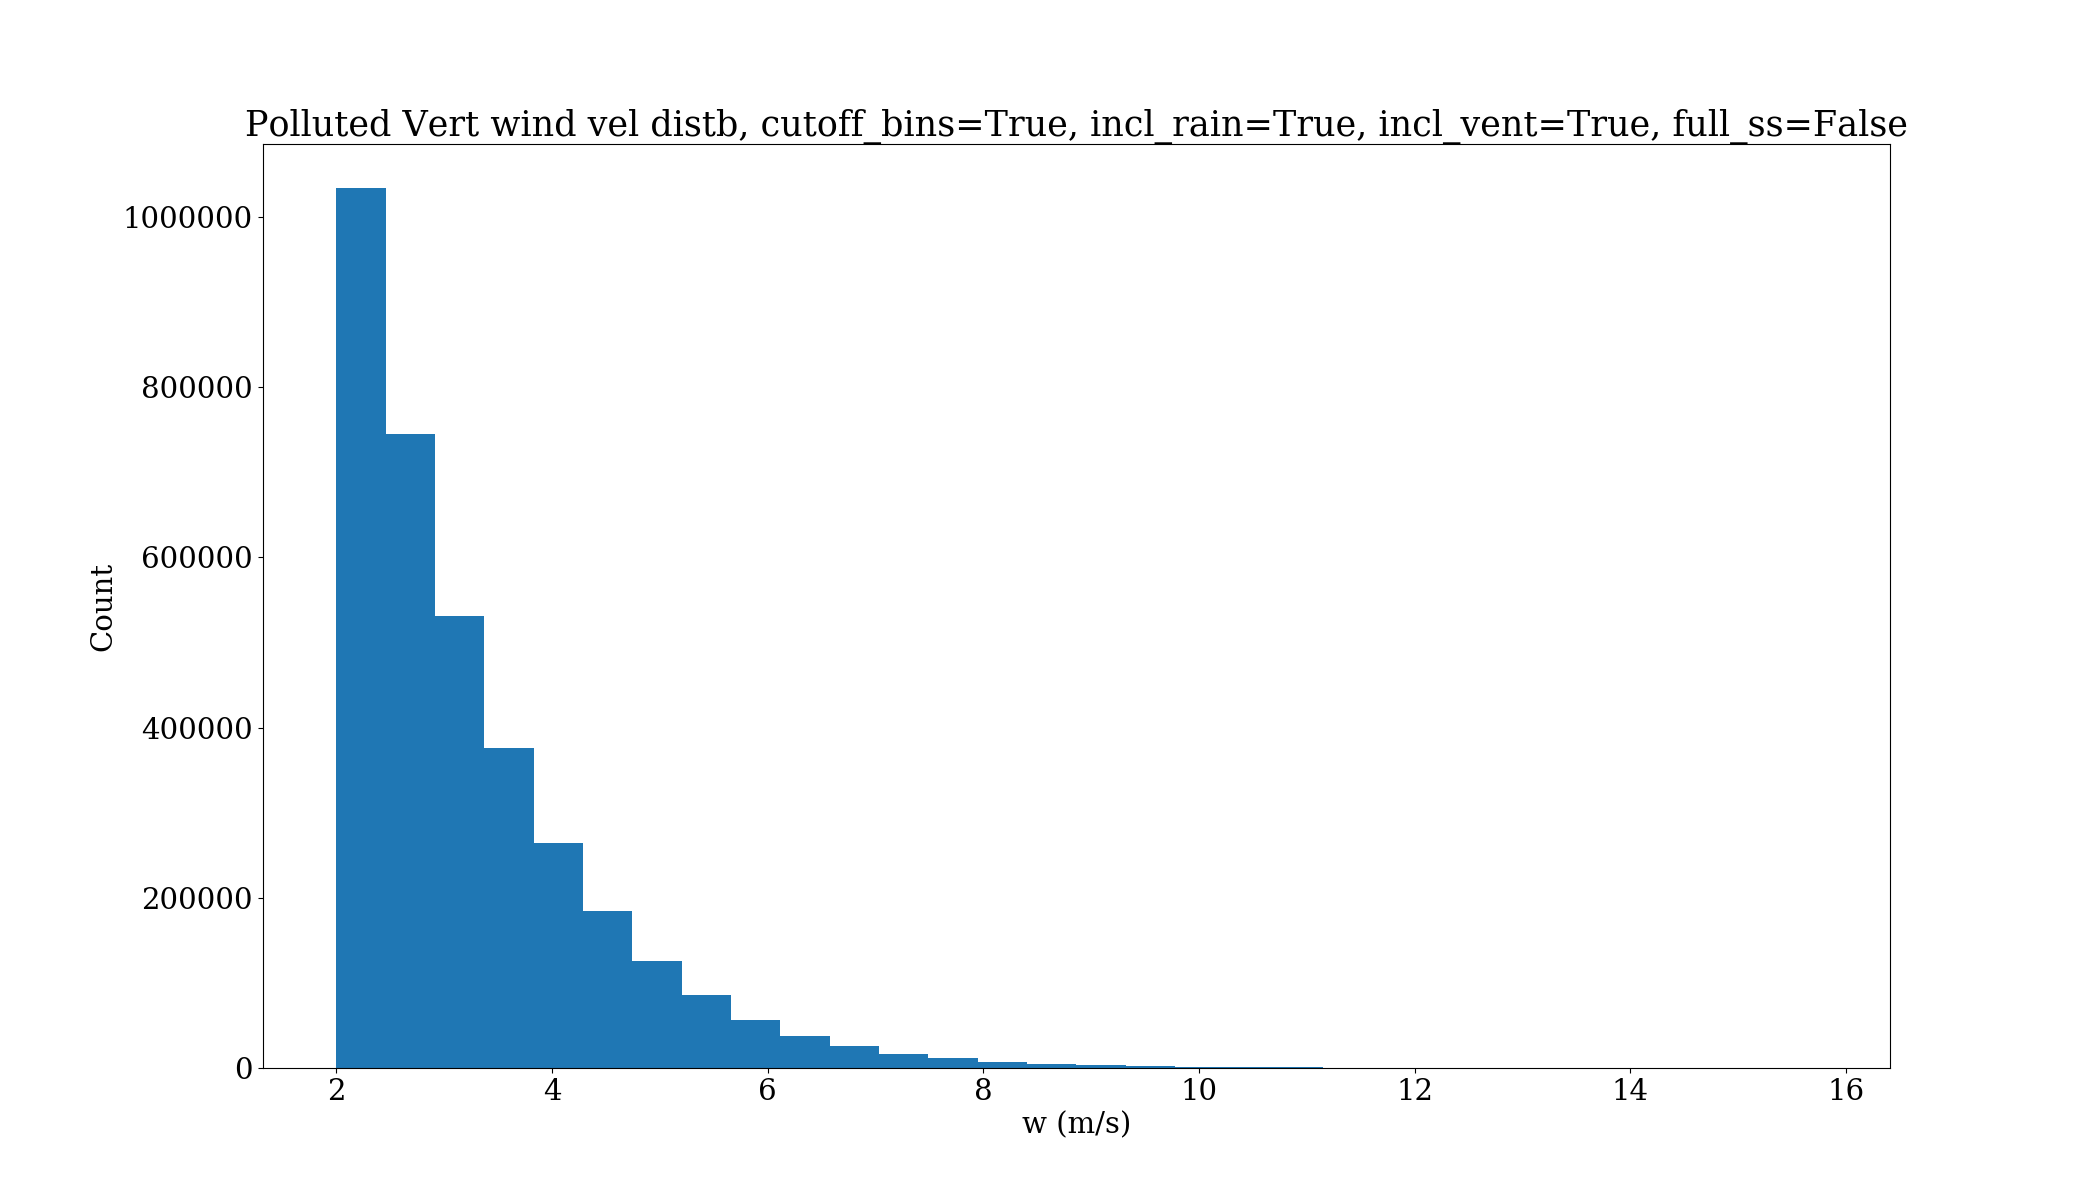
\includegraphics[width=\textwidth]{revmywrf/v9_w_hist_Polluted_figure.png}
		\caption{Polluted case.}
		\label{wrfwhistpoll}
	\end{subfigure}
	\caption{Vertical wind velocity distribution in WRF simulation using filtering criteria described in the text.}
	\label{wrfwhist}
\end{figure}

\clearpage
\newpage

\section{Experimental data}
\begin{itemize}
	\item using criteria from second bullet point of section 2, $SS_{QSS}$ distributions from HALO and CAIPEEX campaigns look like figs \ref{haloqsshist} and \ref{caipeexqsshist}, respectively (note: currently don't have raindrop data for CAIPEEX...). 
	\item using same criteria, cloud LWC distributions are given in figs \ref{halolwchist} and \ref{caipeexlwchist}. 
	\item using same criteria, vertical wind velocity distributions are given in figs \ref{halowhist} and \ref{caipeexwhist}. 
\end{itemize}
\begin{figure}[ht]
    \centering
    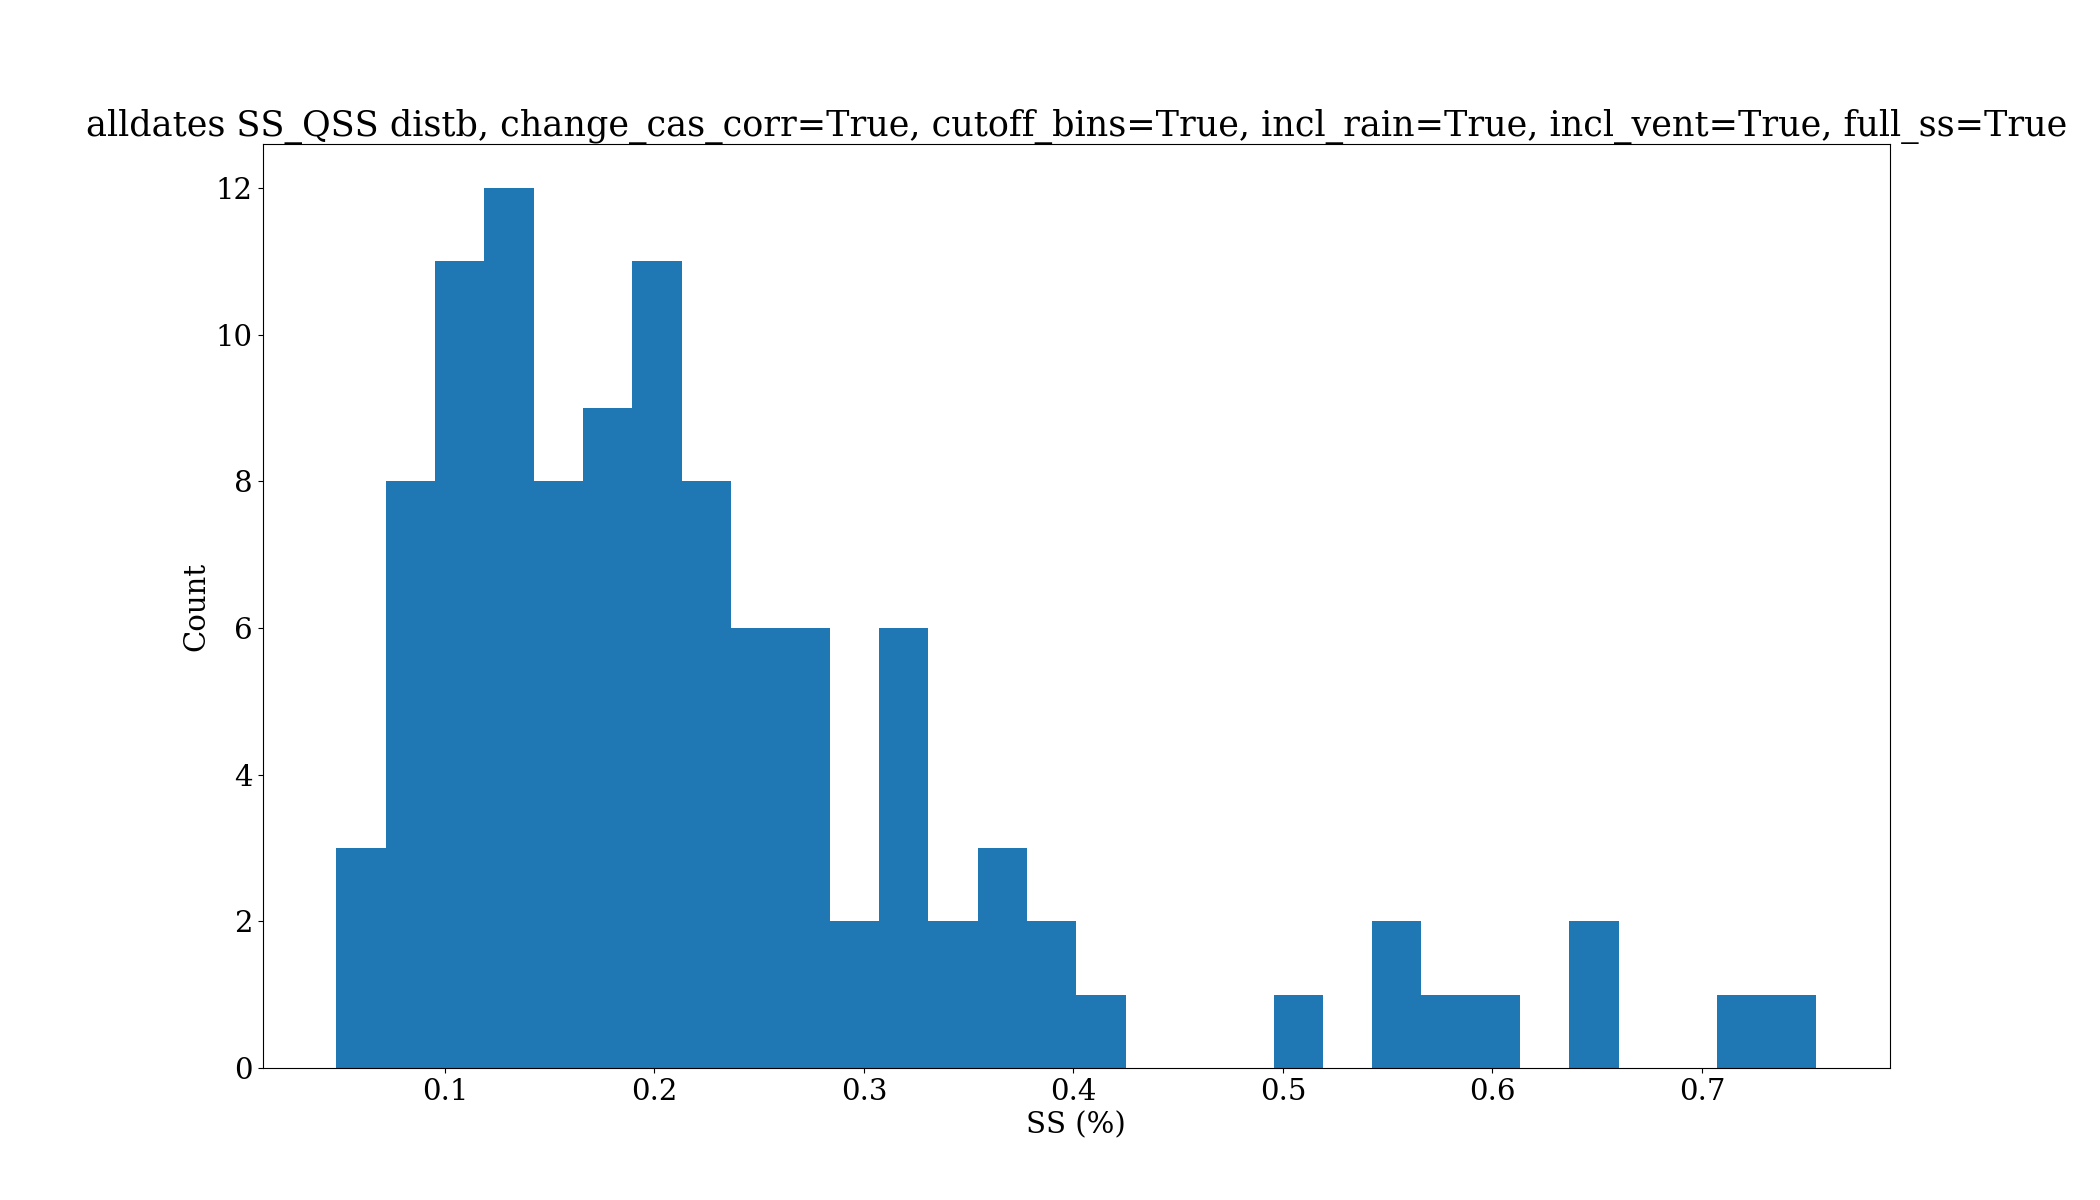
\includegraphics[width=9cm]{revhalo/v24_ss_qss_hist_cas_alldates_figure.png}
    \caption{Predicted ($SS_{QSS}$) supersaturation distribution from HALO field campaign (all flight dates). Using filtering criteria outlined in section 2.}
    \label{haloqsshist}
\end{figure}
\begin{figure}[ht]
    \centering
    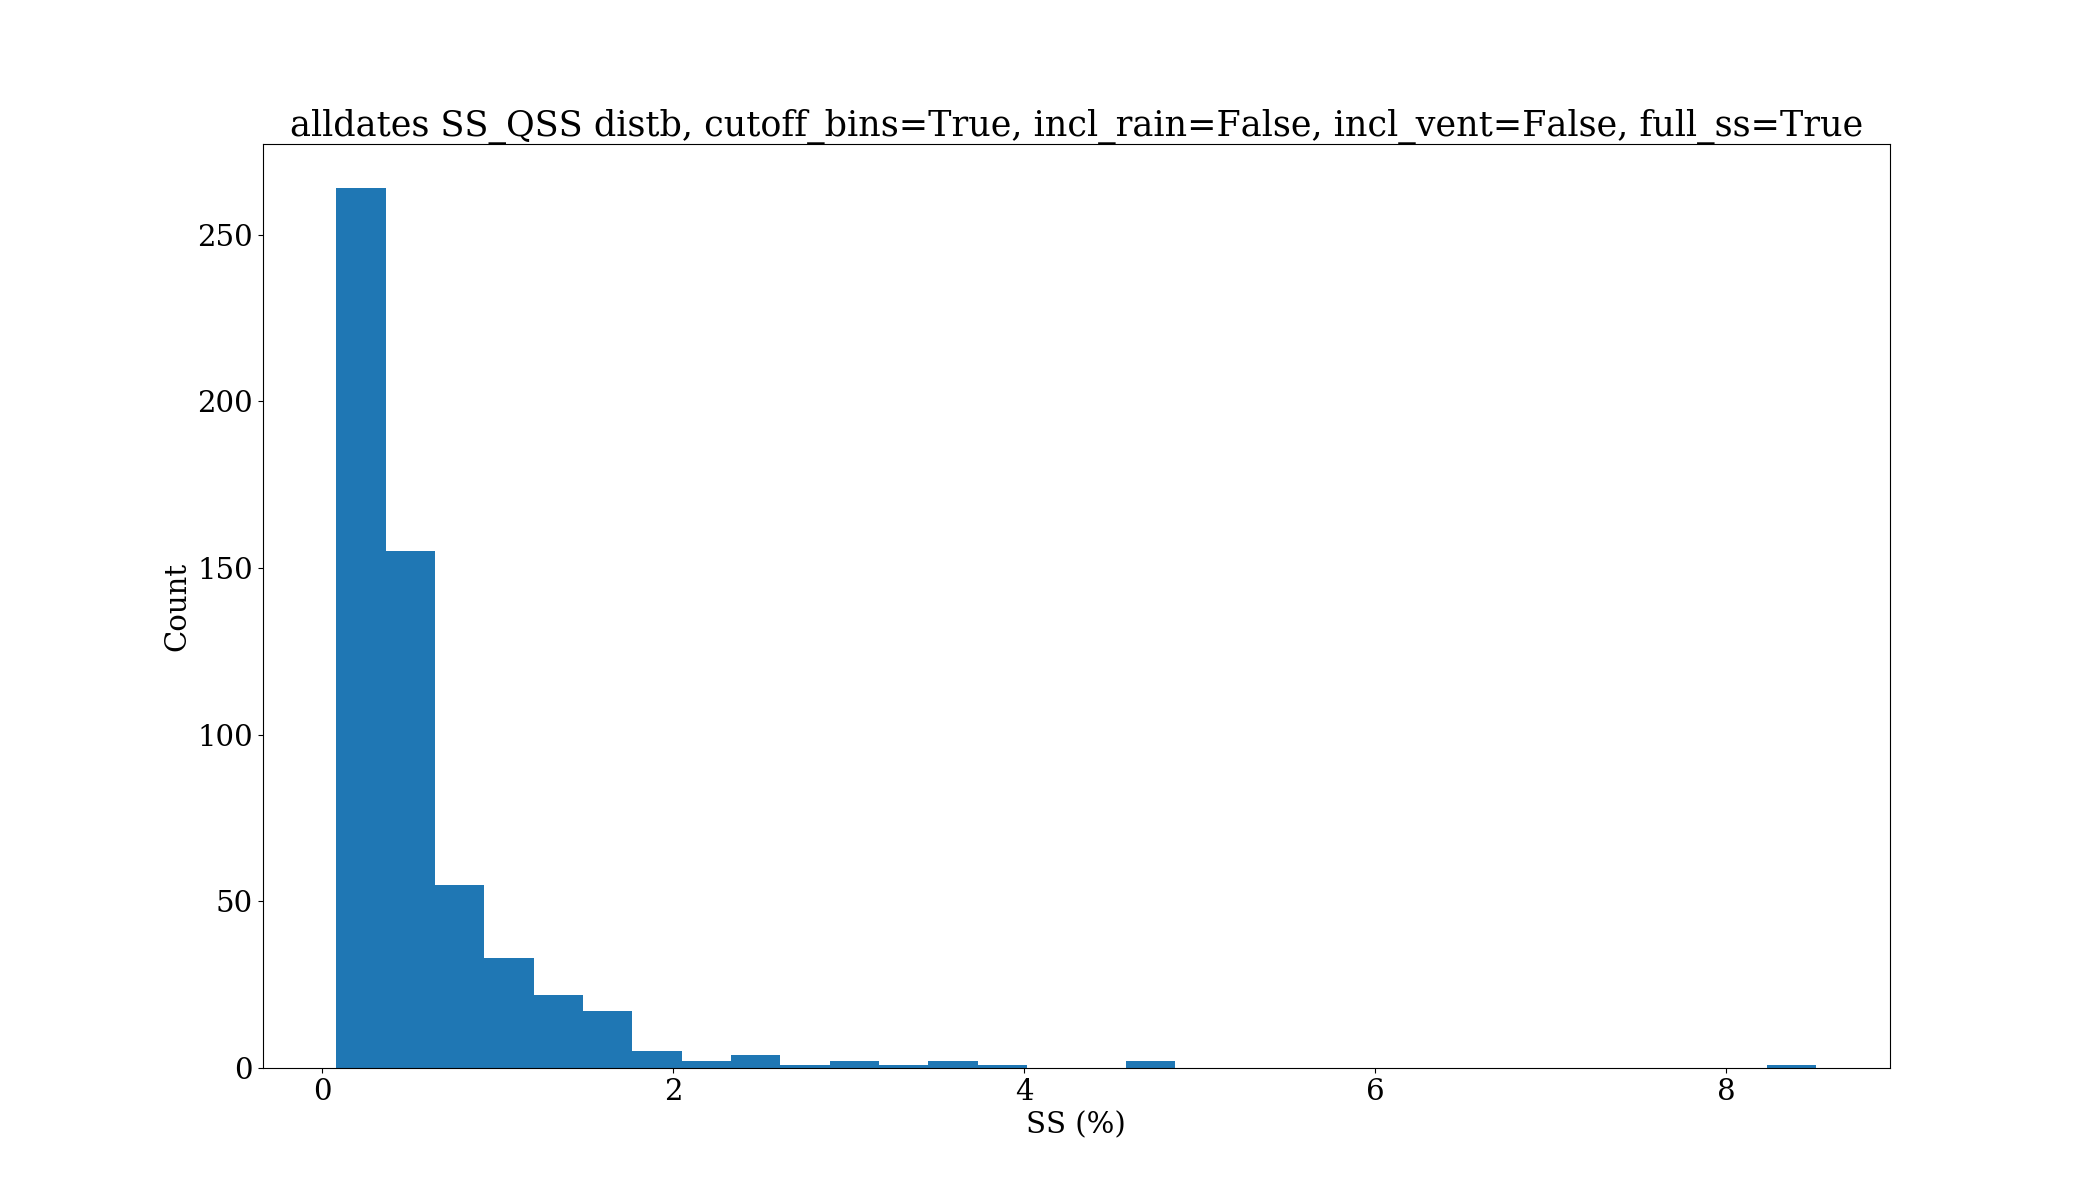
\includegraphics[width=9cm]{revcaipeex/v10_ss_qss_hist_alldates_figure.png}
    \caption{Predicted ($SS_{QSS}$) supersaturation distribution from CAIPEEX field campaign (all flight dates). Using filtering criteria outlined in section 2, but not including rain drops or ventilation corrections due to lack of data.}
    \label{caipeexqsshist}
\end{figure}
\begin{figure}[ht]
    \centering
    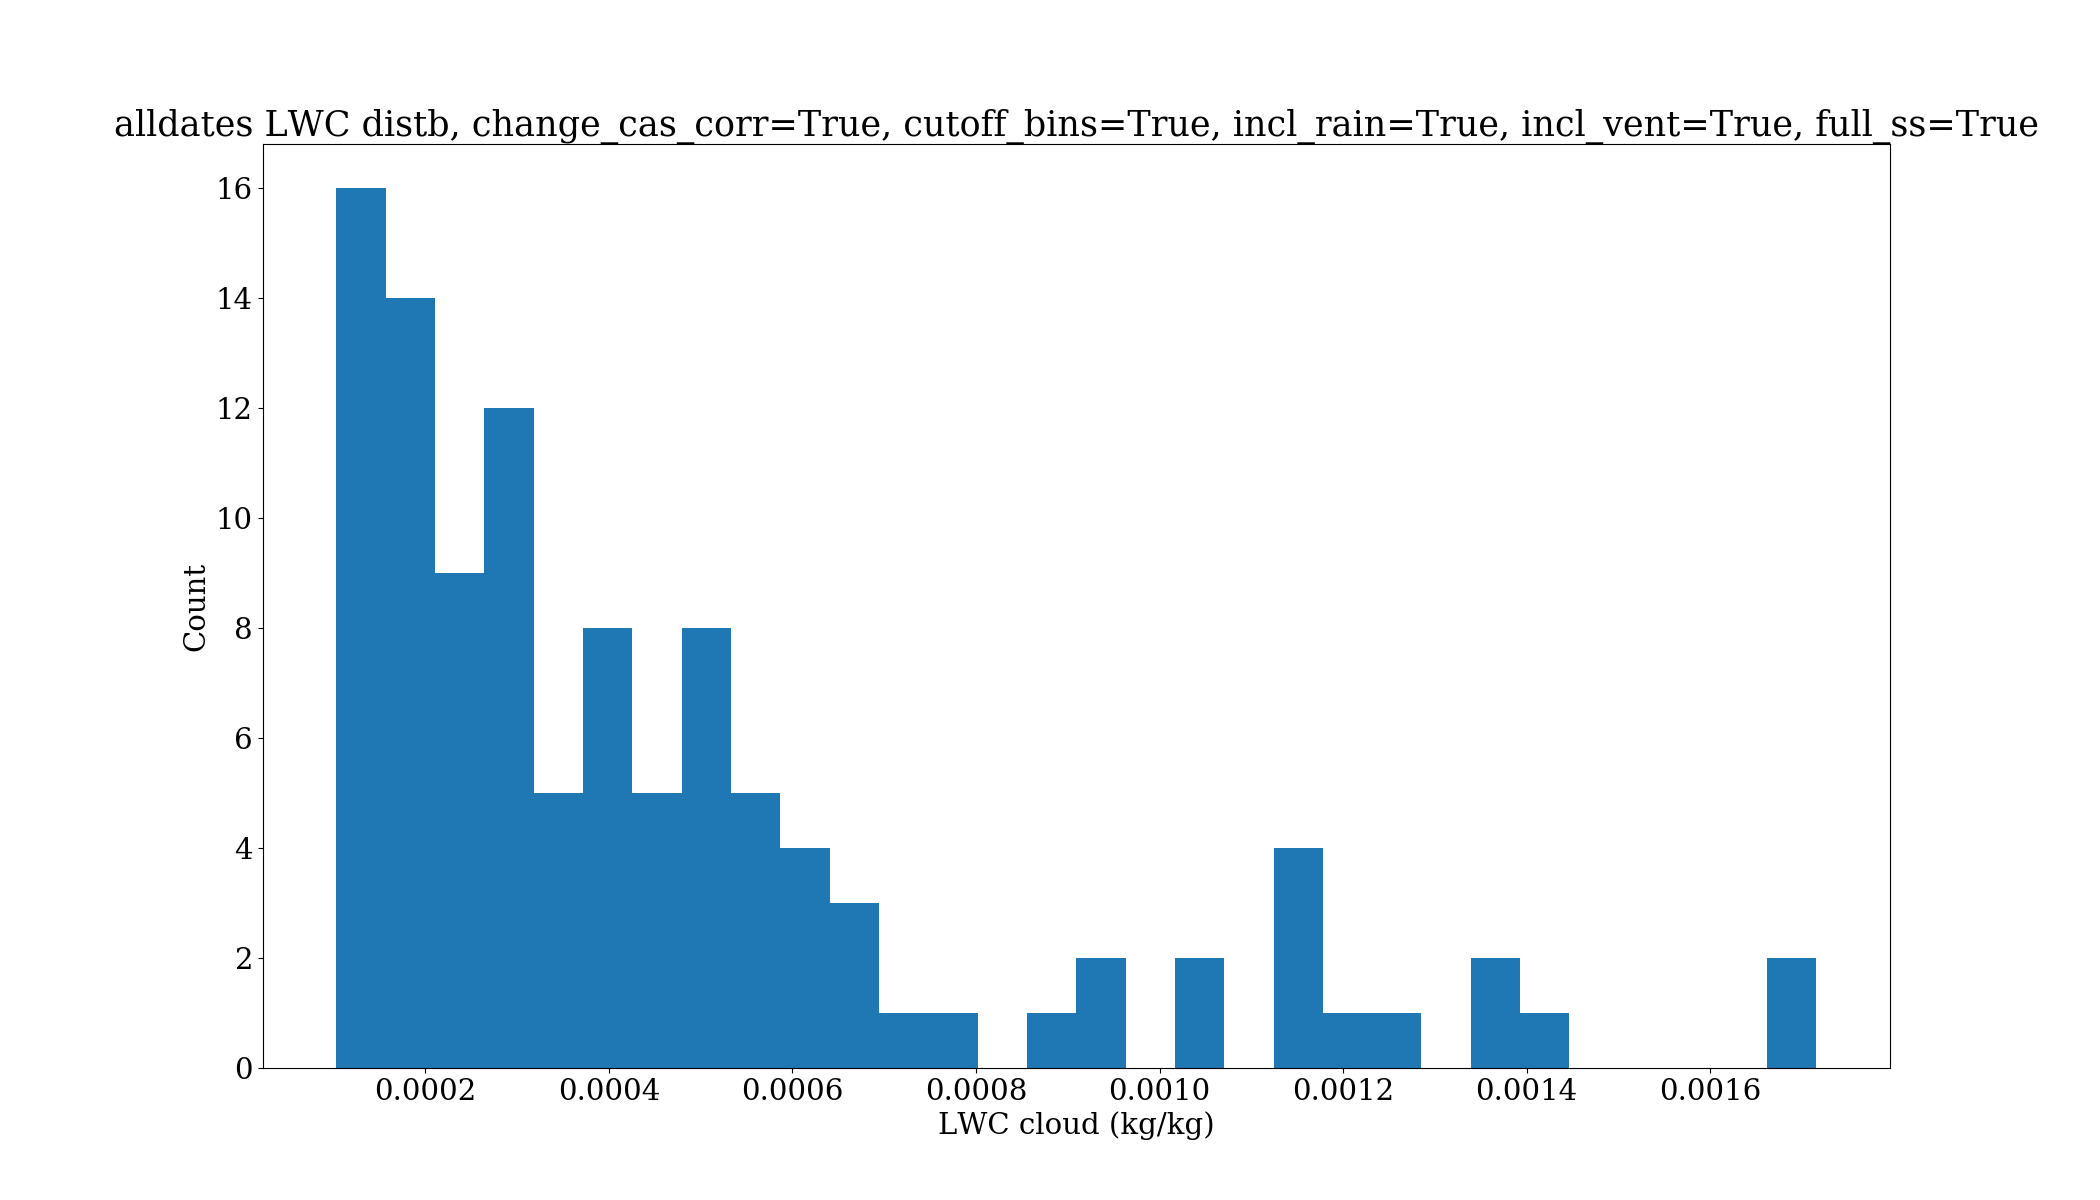
\includegraphics[width=9cm]{revhalo/v24_lwc_hist_cas_alldates_figure.png}
    \caption{Cloud LWC distribution from HALO field campaign (all flight dates). Using filtering criteria outlined in section 2.}
    \label{halolwchist}
\end{figure}
\begin{figure}[ht]
    \centering
    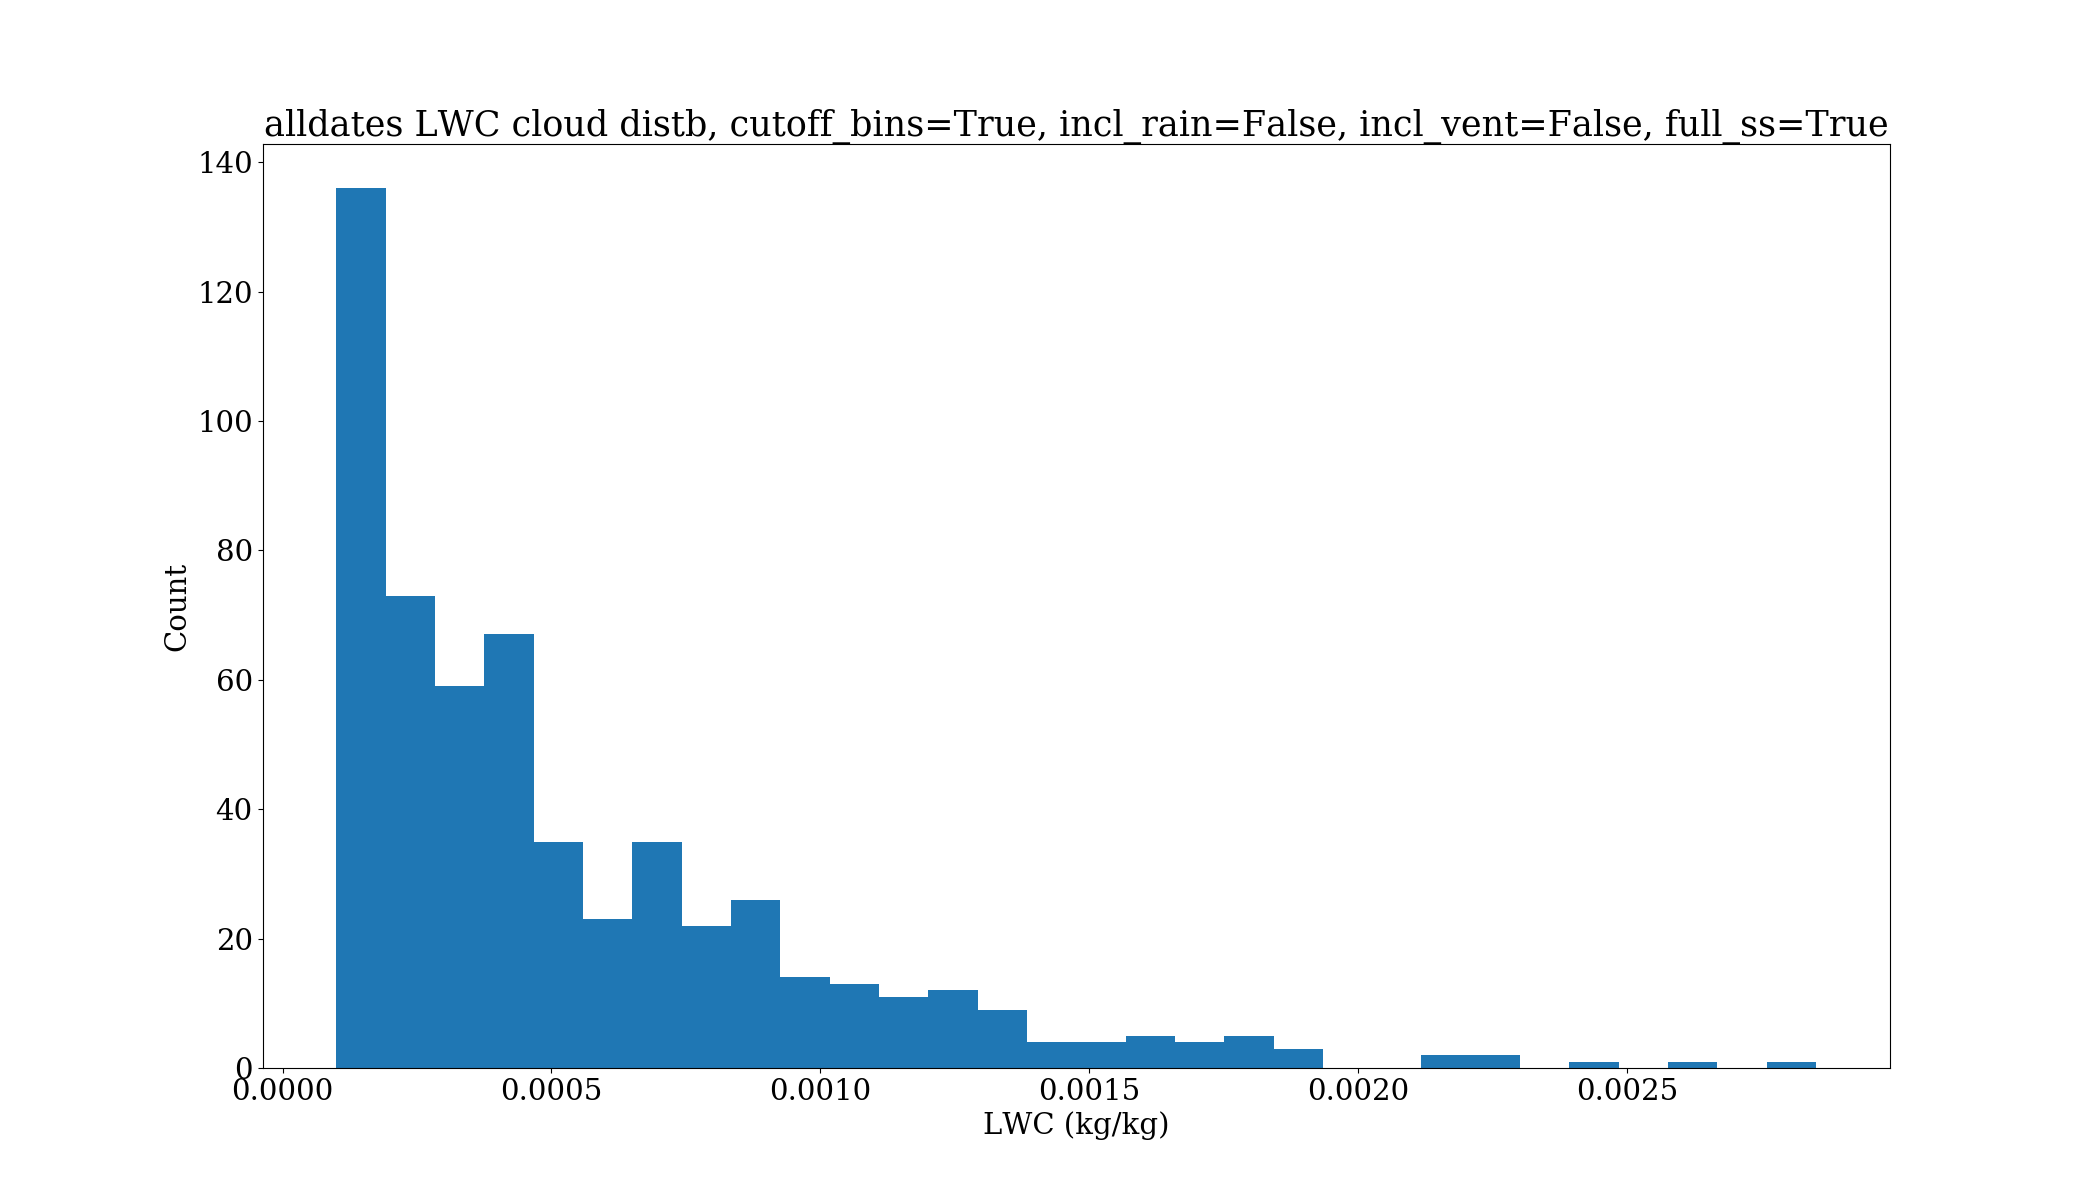
\includegraphics[width=9cm]{revcaipeex/v10_lwc_hist_alldates_figure.png}
    \caption{Cloud LWC distribution from CAIPEEX field campaign (all flight dates). Using filtering criteria outlined in section 2, but not including rain drops or ventilation corrections due to lack of data.}
    \label{caipeexlwchist}
\end{figure}
\begin{figure}[ht]
    \centering
    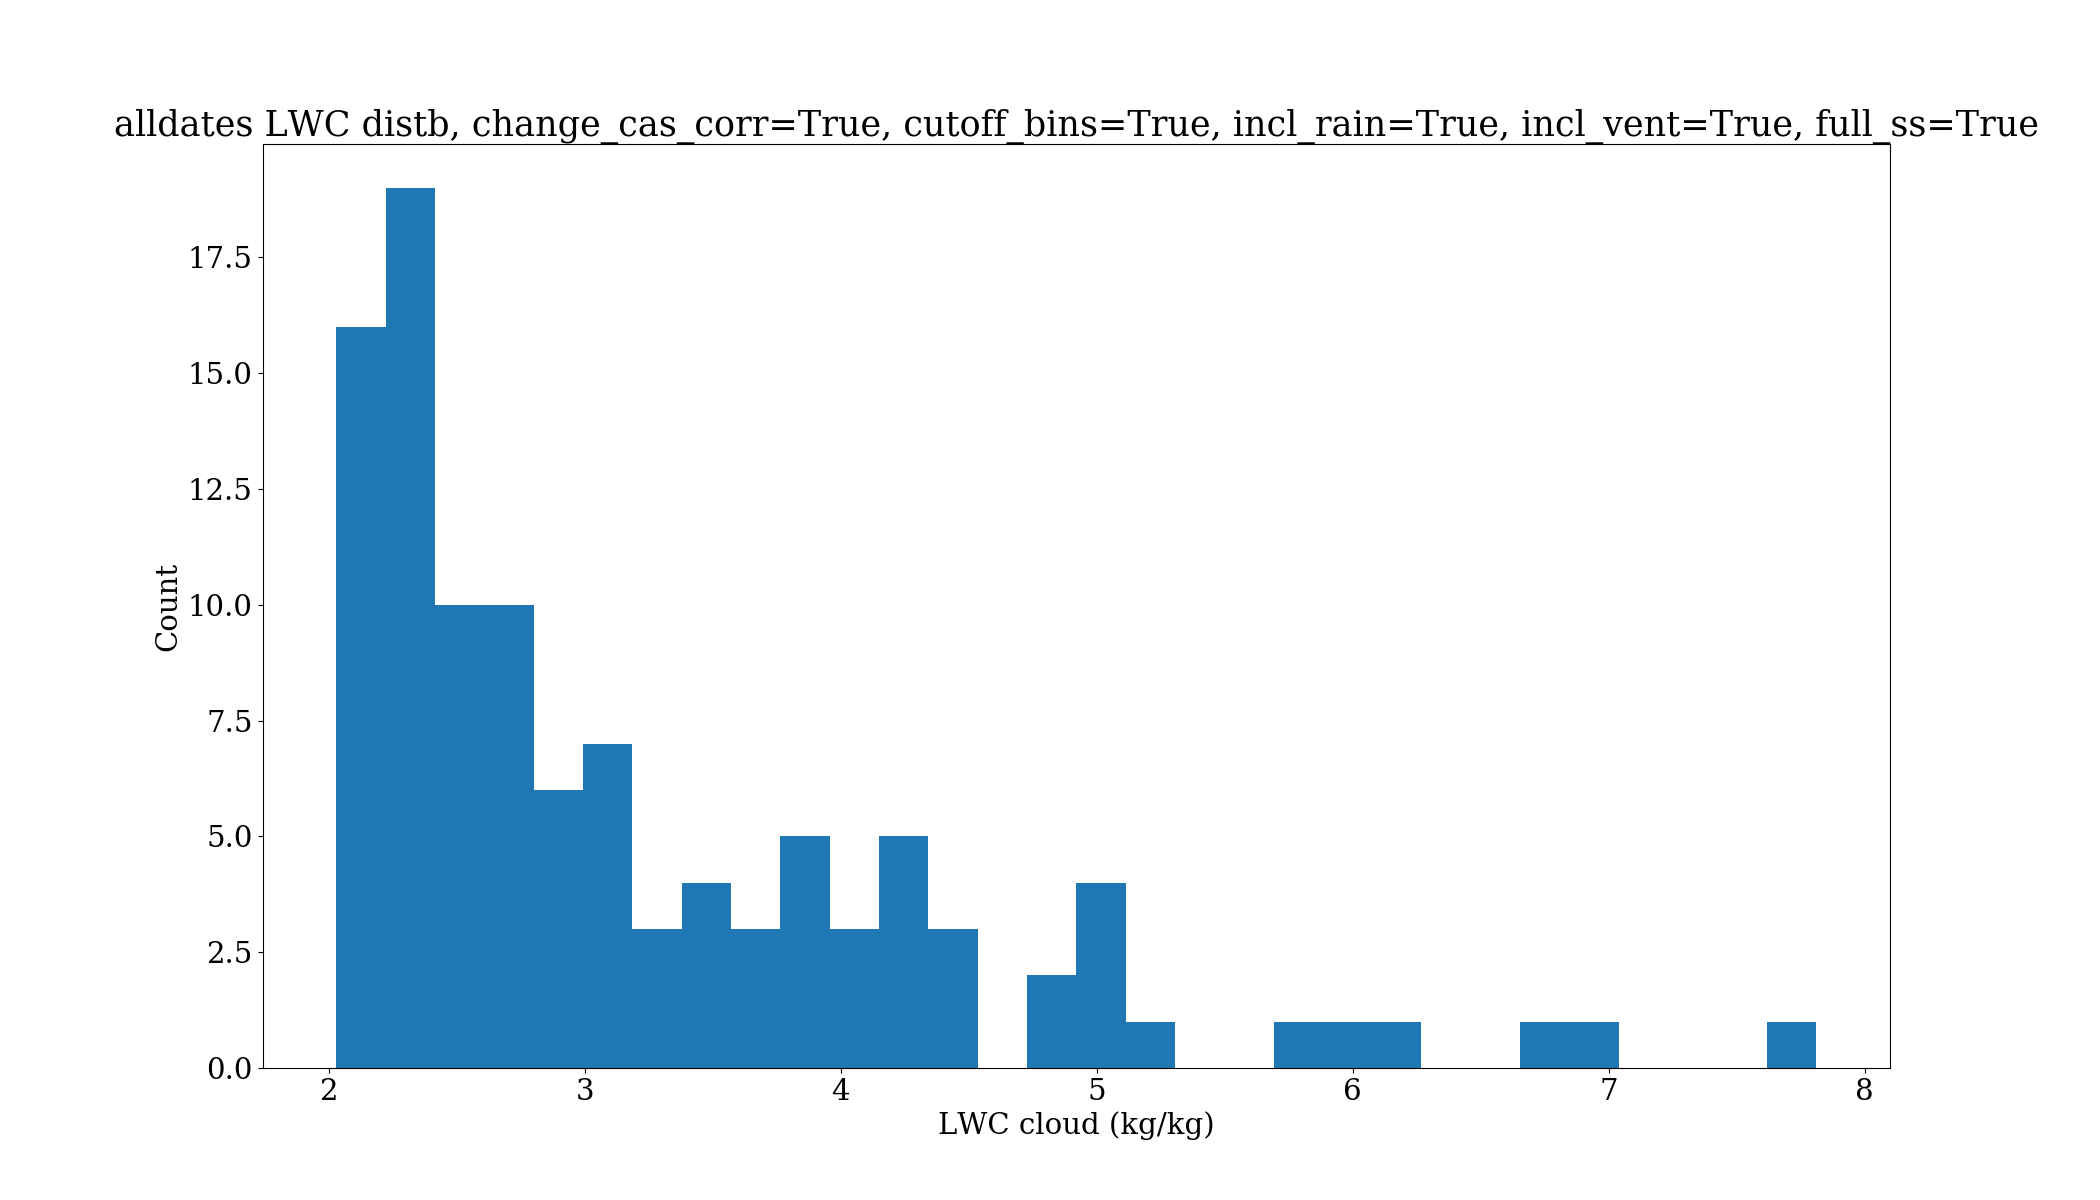
\includegraphics[width=9cm]{revhalo/v24_w_hist_cas_alldates_figure.png}
    \caption{Vertical wind velocity distribution from HALO field campaign (all flight dates). Using filtering criteria outlined in section 2.}
    \label{halowhist}
\end{figure}
\begin{figure}[ht]
    \centering
    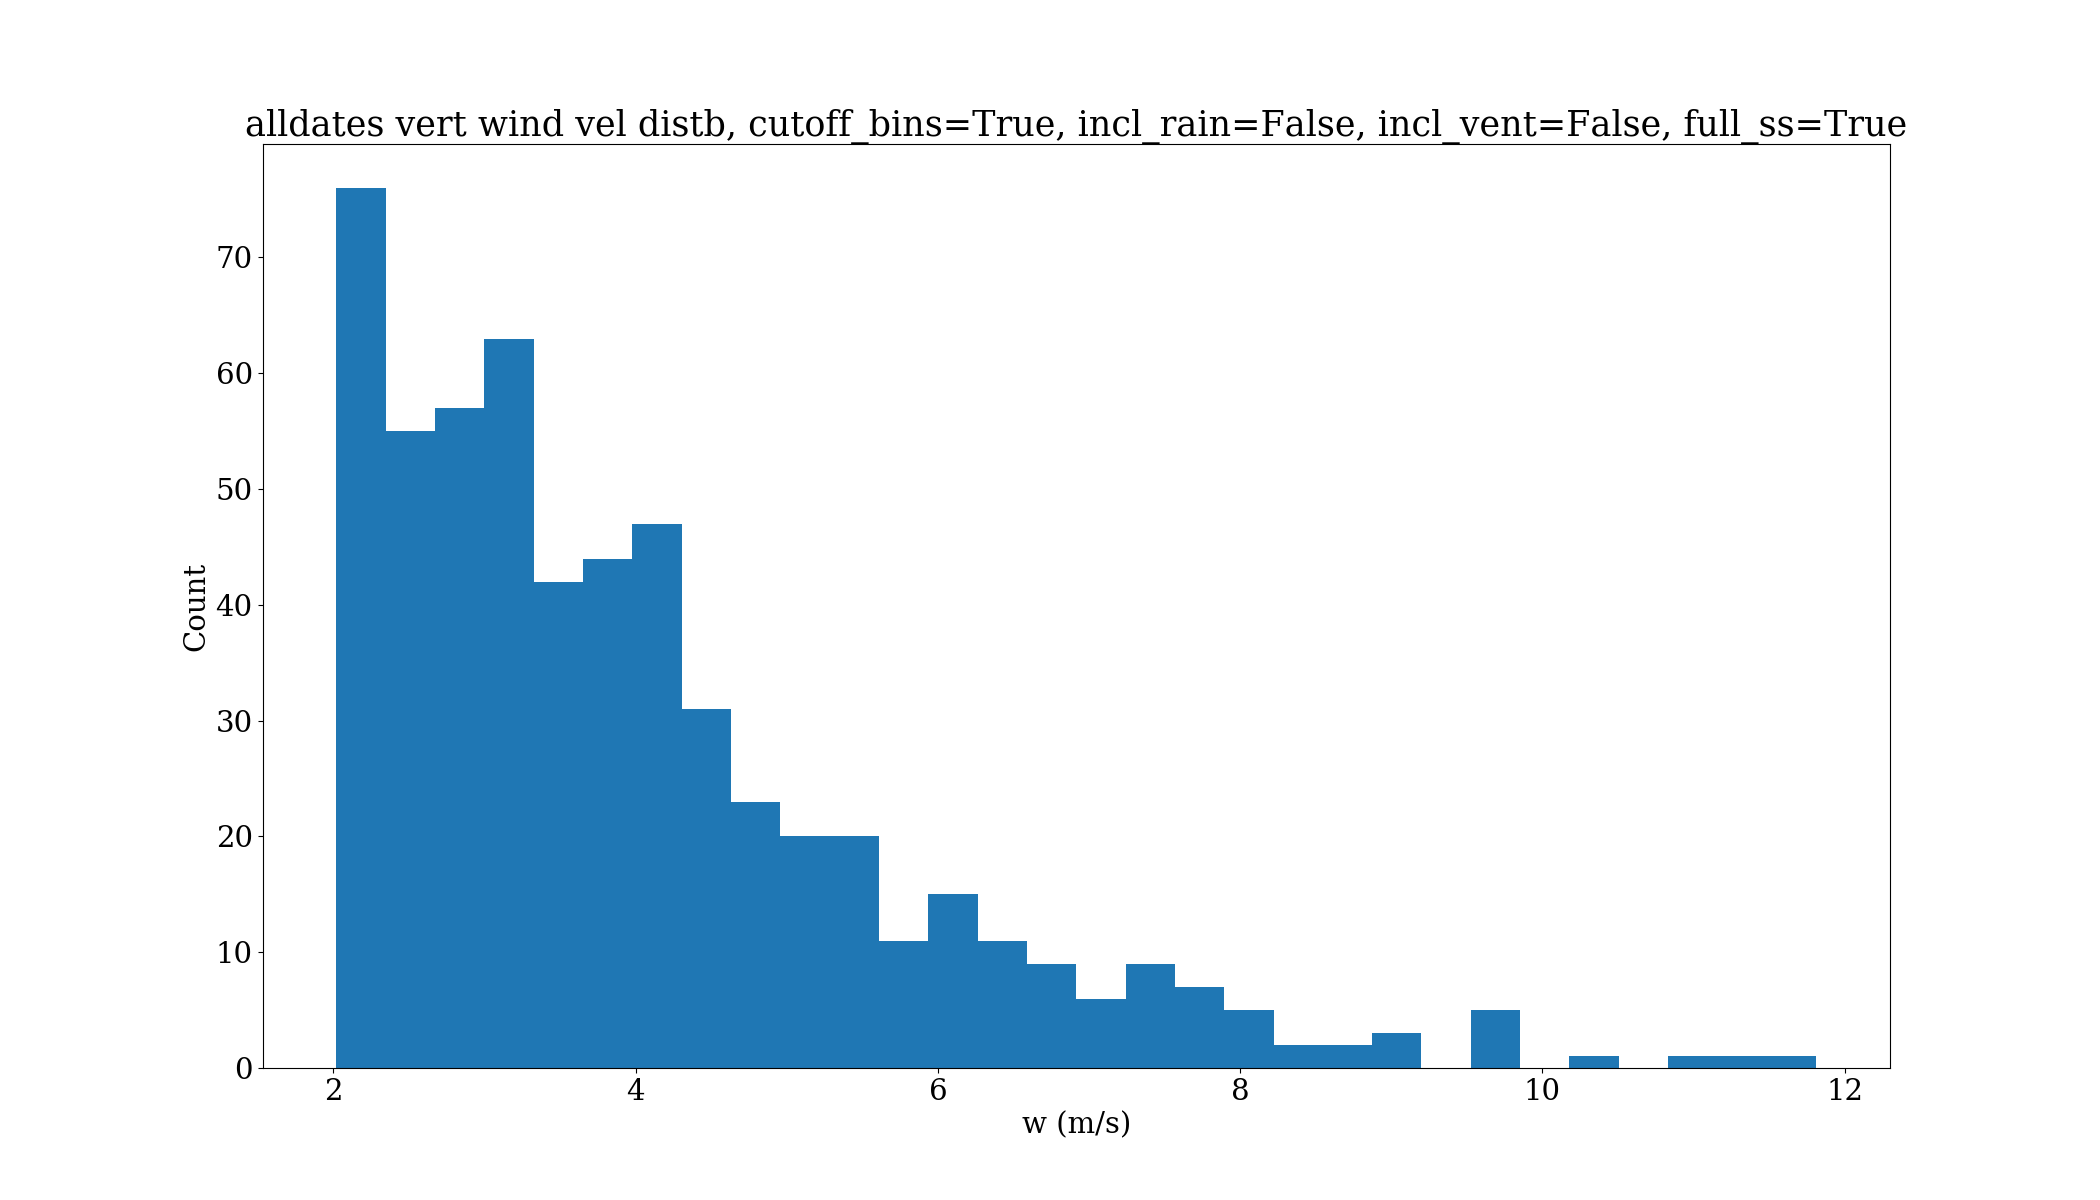
\includegraphics[width=9cm]{revcaipeex/v10_w_hist_alldates_figure.png}
    \caption{Vertical wind velocity distribution from CAIPEEX field campaign (all flight dates). Using filtering criteria outlined in section 2, but not including rain drops or ventilation corrections due to lack of data.}
    \label{caipeexwhist}
\end{figure}

\clearpage
\newpage

\section{Line of argument}
\subsection{CLAIM}
Figures \ref{haloqsshist} and \ref{caipeexqsshist} demonstrate that we don't observe the same high supersaturations seen in LES simulations (i.e. WRF data) 
\subsection{POSSIBLE COUNTERARGUMENTS}
\begin{enumerate}
	\item Experimental sites were too polluted to observe the high supersaturations
	\item Something must be wrong because $SS_{QSS}$ distributions are so different between HALO and CAIPPEX.
	\item (more philosophical I guess) If you don't trust WRF to give you realistic supersaturation values then why do you trust it to give you the reasonable regime of validity for the QSS approximation?
\end{enumerate}
\subsection{POSSIBLE COUNTERARGUMENTS TO THE POSSIBLE COUNTERARGUMENTS}
\begin{enumerate}
	\item Compare experiment vs simulation for **mystery kernel** integrated over aerosol distribution. For now I am setting mystery kernel = 1 (i.e. final integrated quantity is just the number concentration) and plotting distributions for HALO in fig \ref{haloaerohist}, and for WRF in fig \ref{wrfaeronconchist}. CAIPEEX figure is pending data from Thara. Right now the disparities in form of distributions is due to different diameter ranges (discuss w/ David).
	\item Ideally the figures referenced in above point will also address this concern, but hard to say right now w/o CAIPEEX aerosol data. Also not sure if we'll have the necessary info based on literature (also a point to discuss) 
	\item Not sure yet...
\end{enumerate}
\begin{figure}[ht]
    \centering
    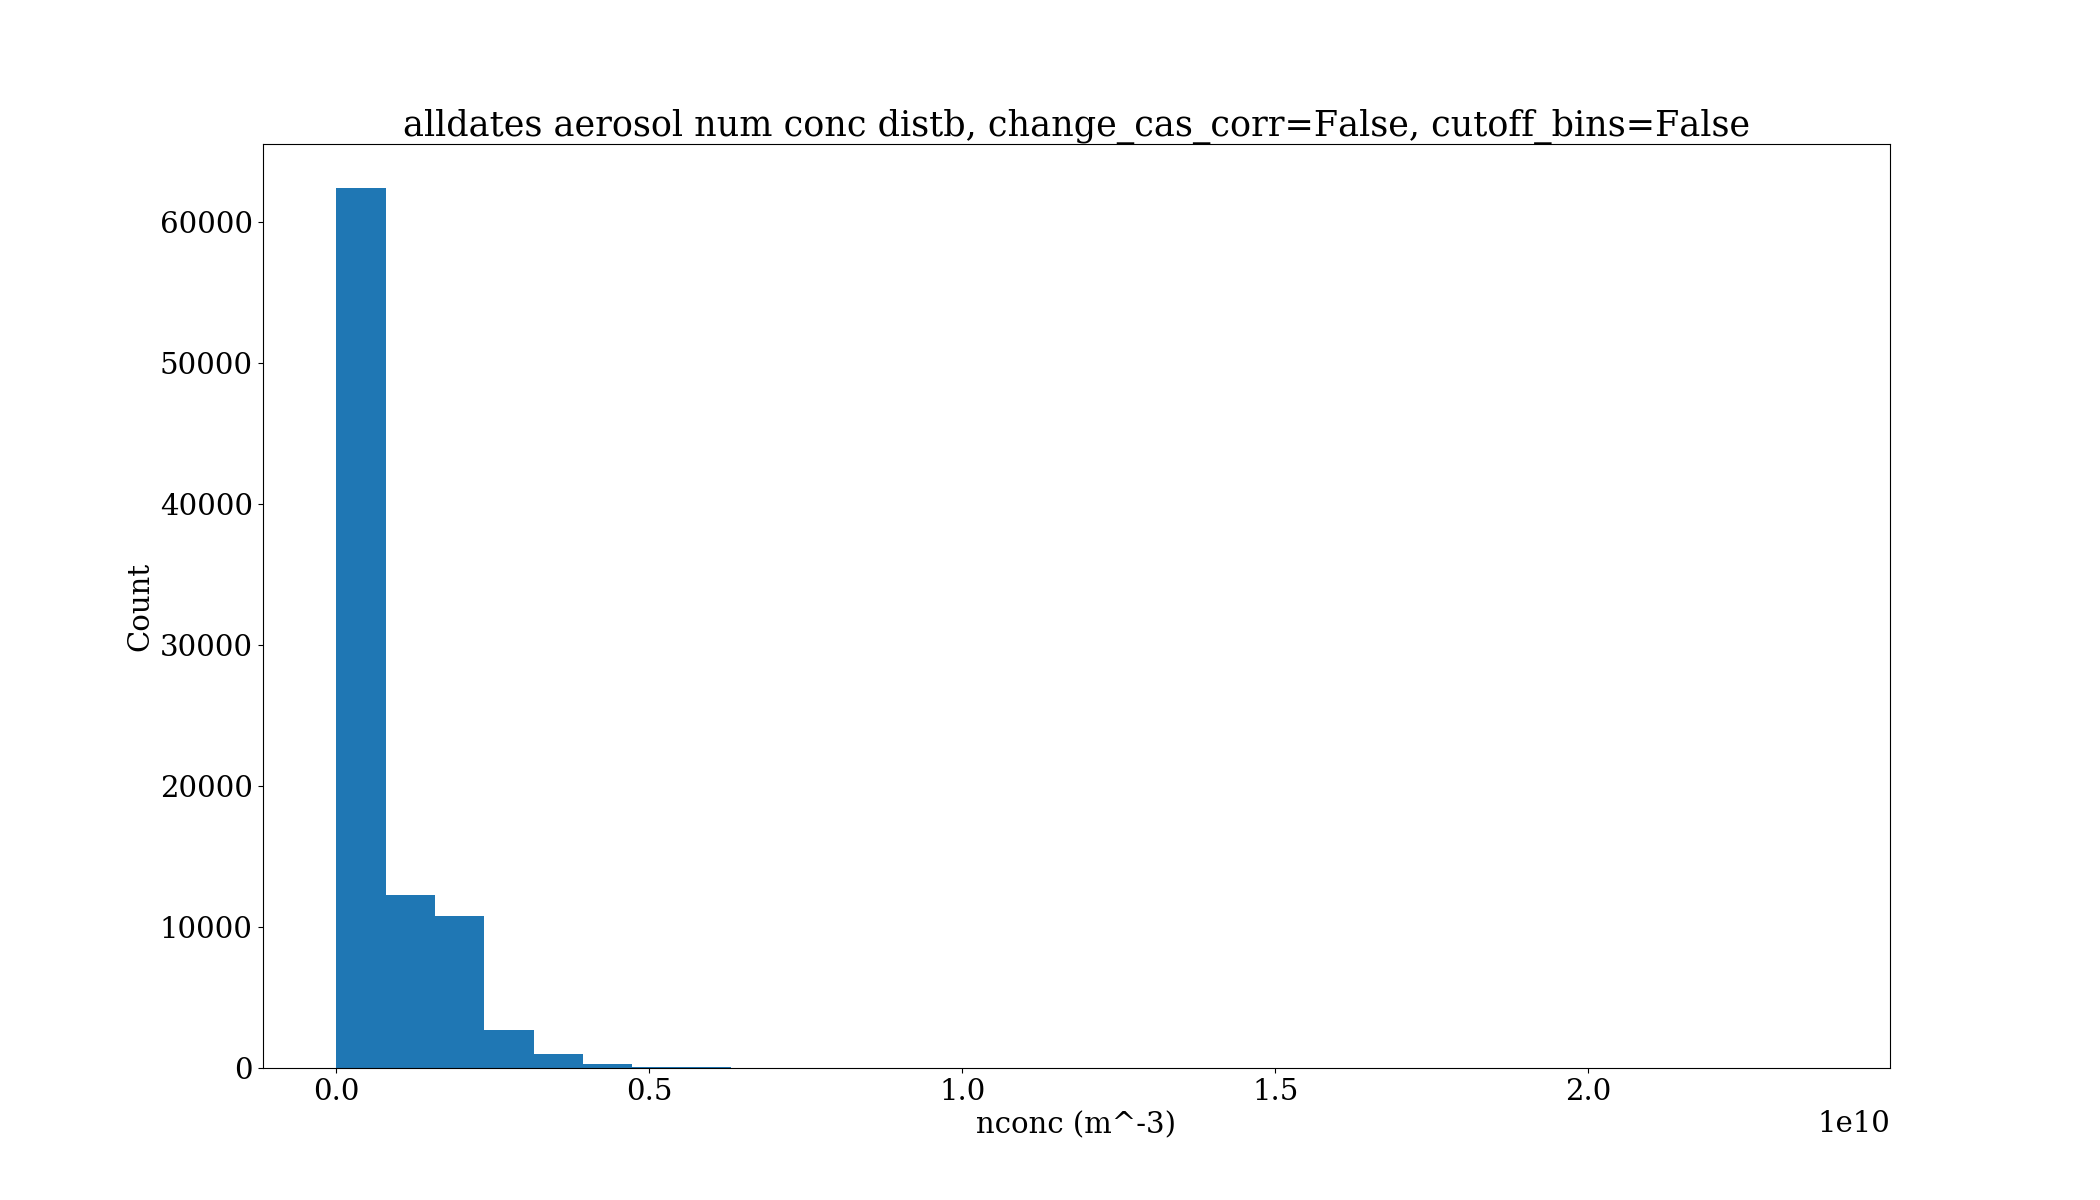
\includegraphics[width=9cm]{revhalo/v1_aero_nconc_hist_cas_alldates_figure.png}
    \caption{Aerosol number concentration distribution for particles 0.1-3.0um in HALO field campaign. All points below the freezing level and have cloud LWC less than 1e-5.}
    \label{haloaerohist}
\end{figure}
\begin{figure}[ht]
	\centering
	\begin{subfigure}{0.7\textwidth}
		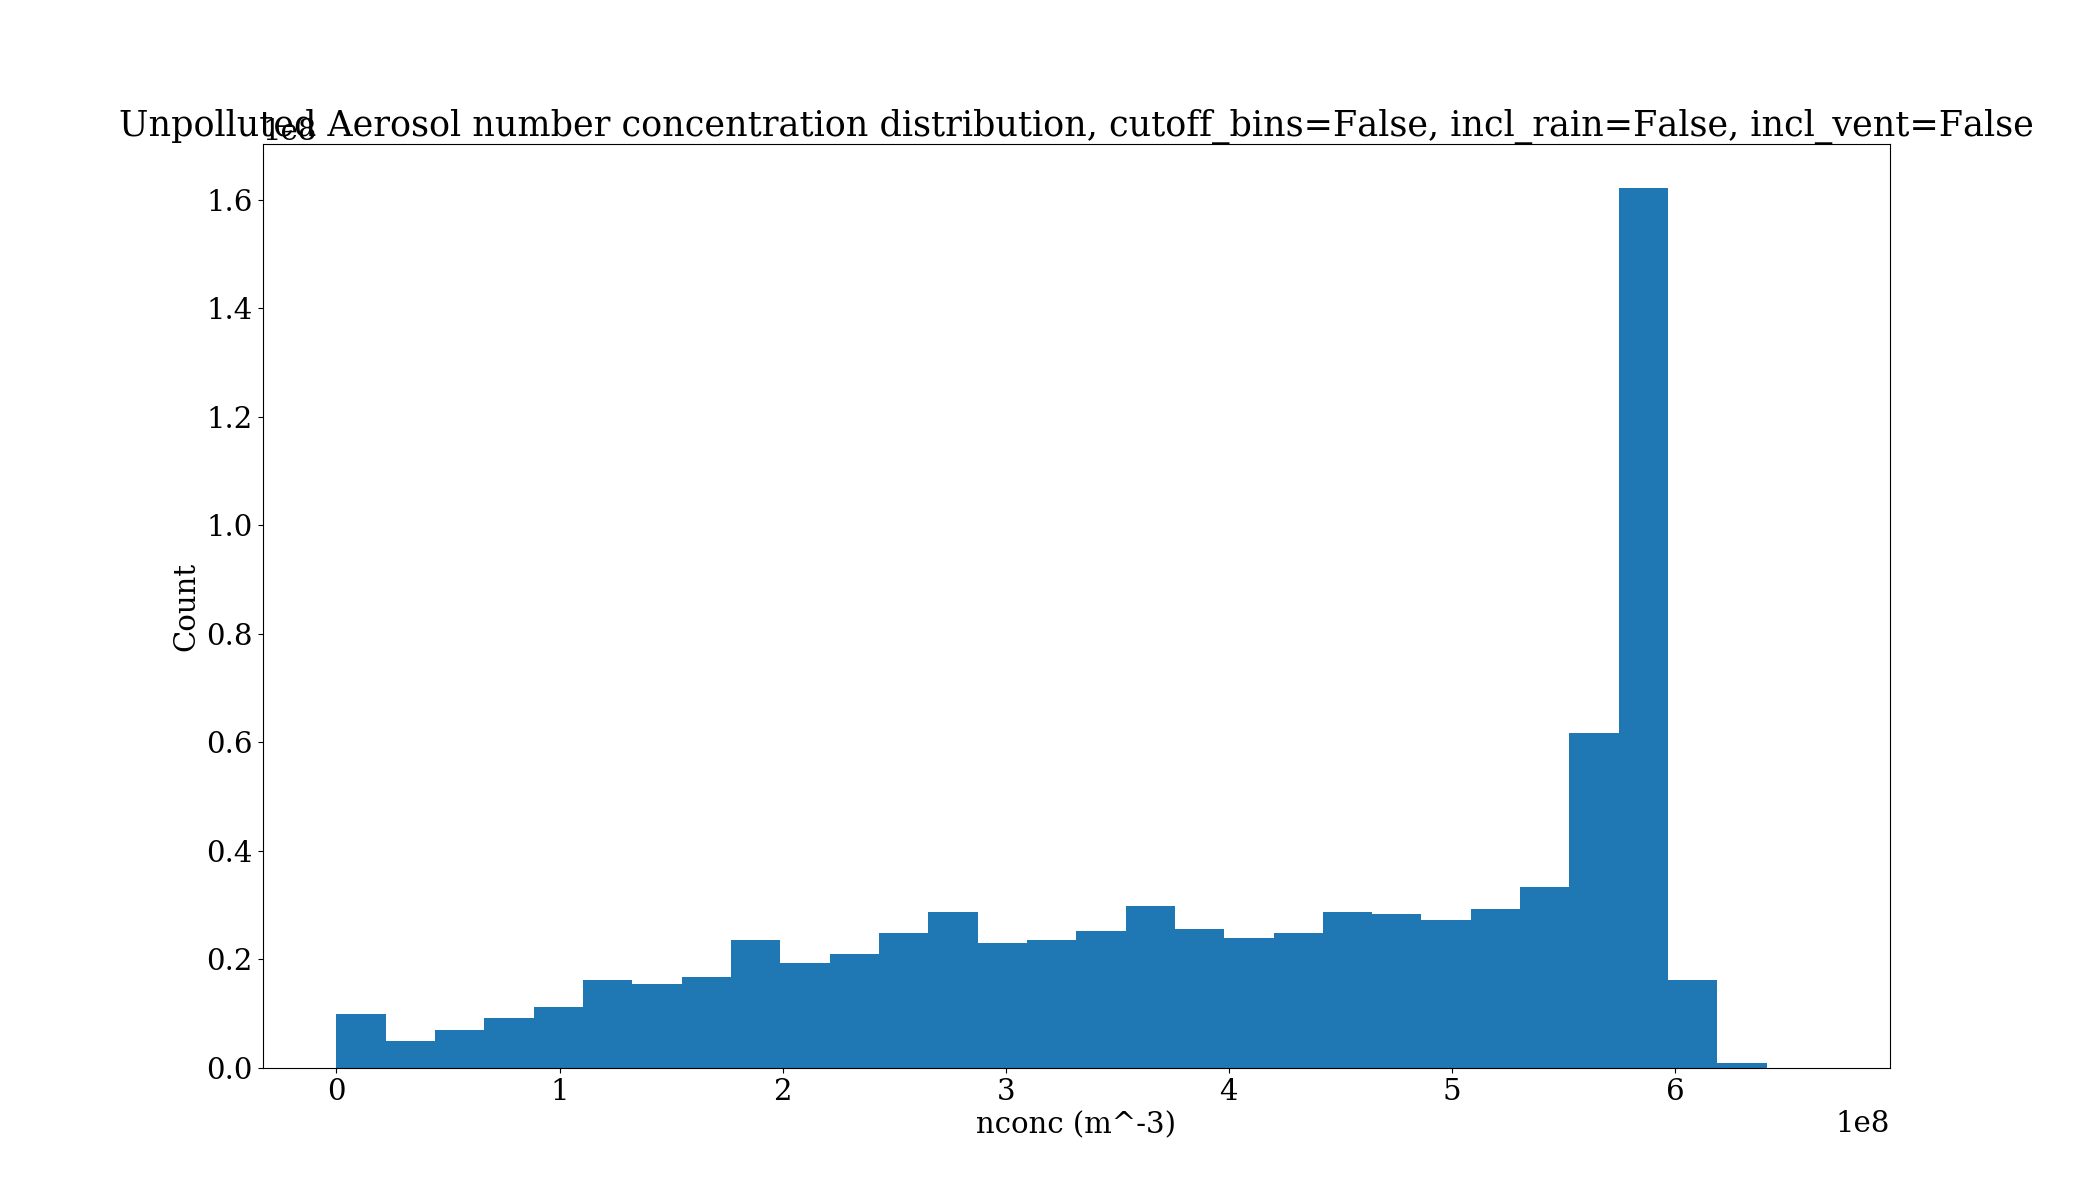
\includegraphics[width=\textwidth]{revmywrf/v1_aero_nconc_hist_Unpolluted_figure.png}
		\caption{Unpolluted case.}
		\label{wrfaeronconchistunpoll}
	\end{subfigure}
	\begin{subfigure}{0.7\textwidth}
		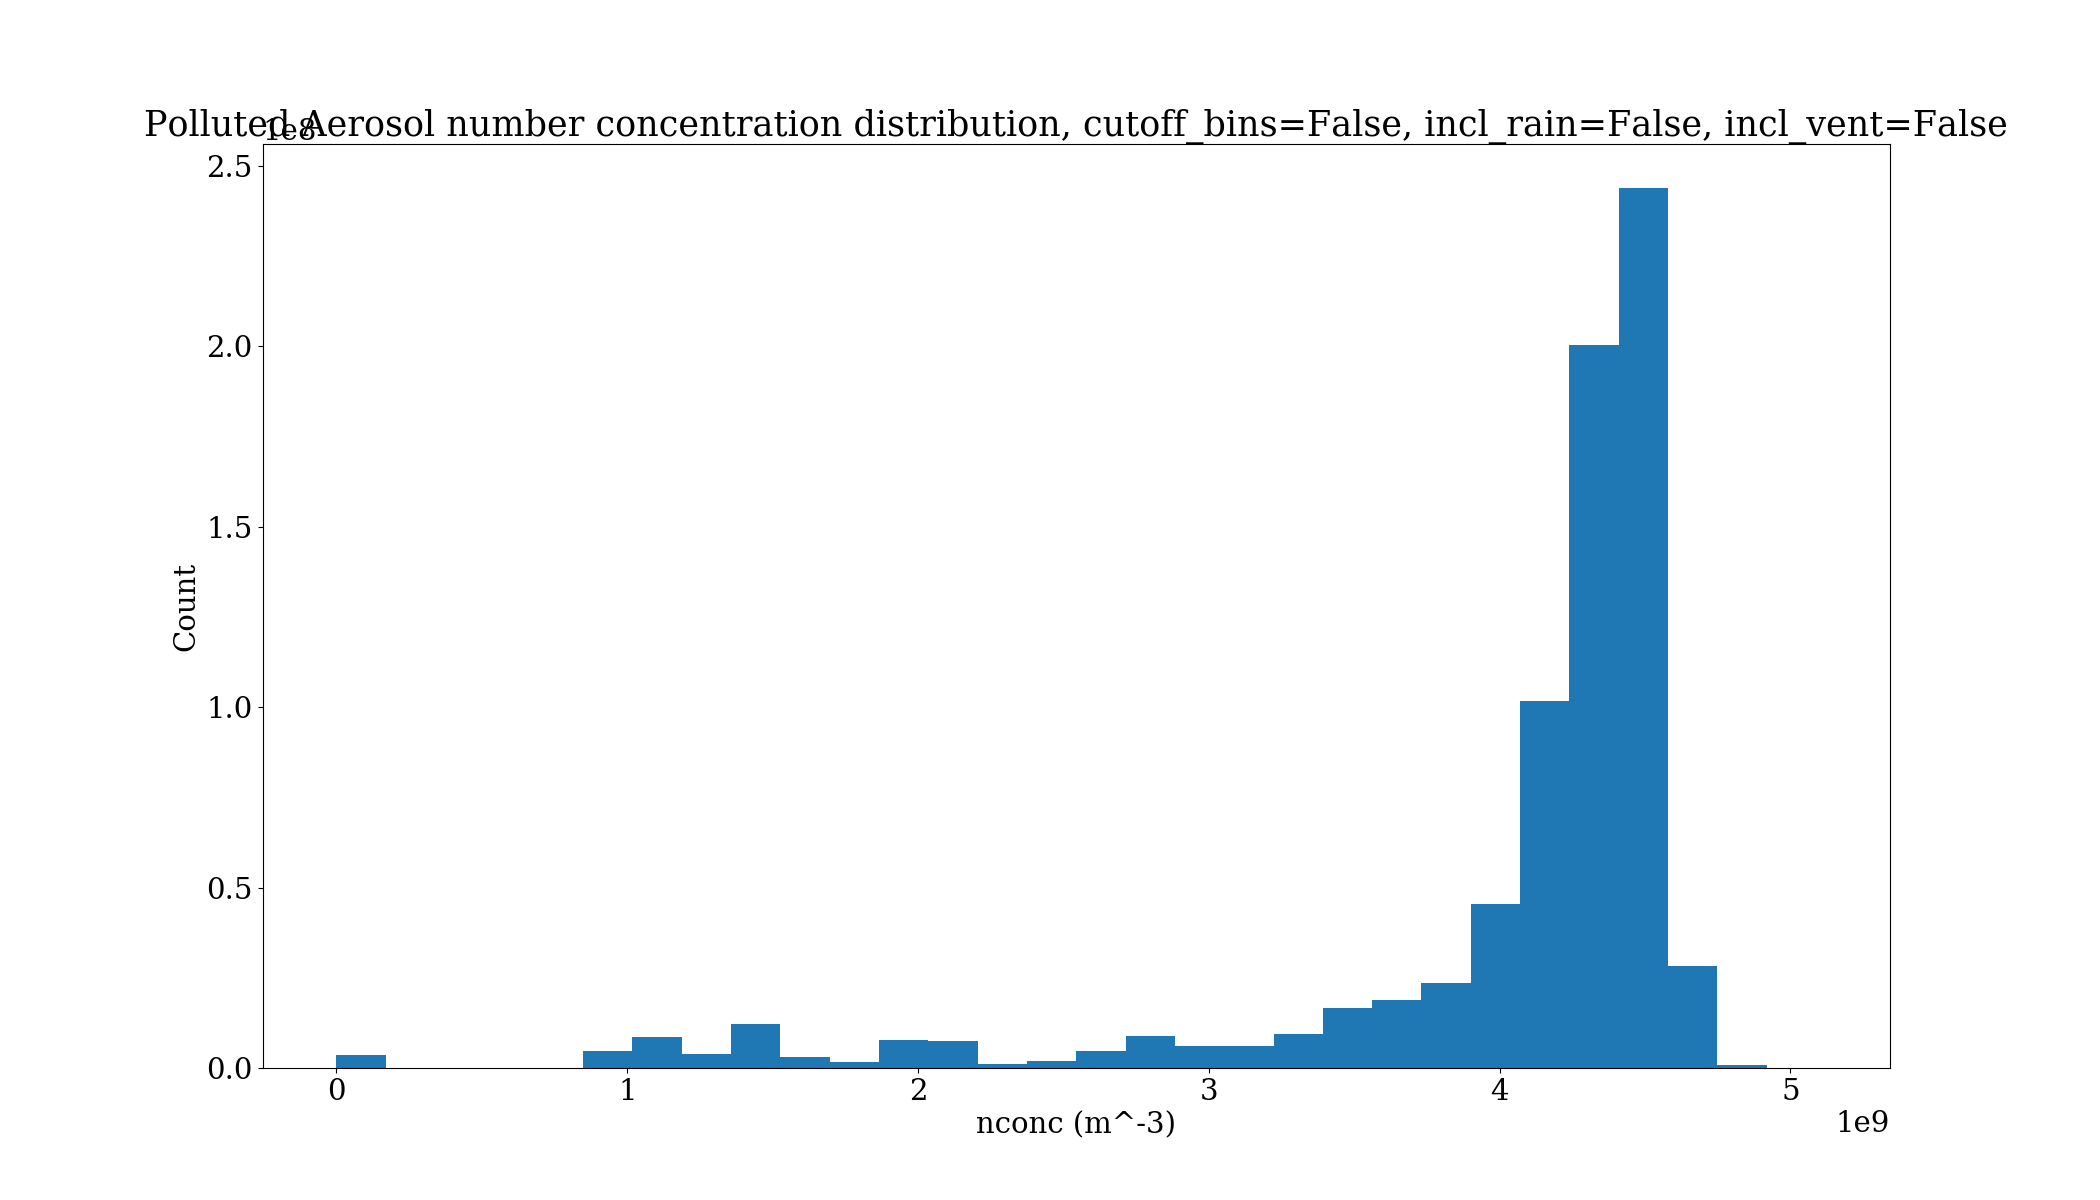
\includegraphics[width=\textwidth]{revmywrf/v1_aero_nconc_hist_Polluted_figure.png}
		\caption{Polluted case.}
		\label{wrfaeronconchistpoll}
	\end{subfigure}
	\caption{Aerosol (unknown diam range ?!?) number concentration distribution in WRF simulation, in clear sky regions (cloud LWC less than 1e-5) and below freezing level.}
	\label{wrfaeronconchist}
\end{figure}

\subsection{Statistical analysis of supersaturation distributions}
\subsubsection{Null hypothesis}
Quasi-steady-state supersaturation values at selected sample of points from field campaigns are drawn from a ``true'' distribution like one of the ones from WRF. 
\subsubsection{Test}
Reduced chi-squared
\subsubsection{Details}
Since altitude shows non-negligible correlation with $SS_{QSS}$ in WRF data (Figure \ref{wrfssqssvsz}), we actually need to compare the experimental $SS_{QSS}$ distribution to an adjusted simulated distribution, to account for the differences in altitude distributions for sampled points in both datasets. Specifically:
\begin{equation}
\tilde\chi^2 = \frac{1}{d}\Big(\sum_{k} \frac{(\mathcal{O}_k - E_k)^2}{E_k}\Big),
\end{equation}
where $k$ labels discrete bins into which we group supersaturation values and,
\begin{align}
\mathcal{O}_k &= \text{# of measurements observed in bin $k$ (for all flight dates combined)}\nonumber\\
E_k &= \text{# of measurements observed in bin $k$ (under adjusted $SS_{QSS}$ distribution $P'_{sim}(SS_k)$)}\nonumber
\end{align}
The adjusted distribution is given by:
\begin{equation}
P'_{sim}(SS_k) = \sum_{j} P'_{sim}(z_j, SS_k),
\end{equation}
where,
\begin{equation}
P'_{sim}(z_j, SS_k) = \sum_{k''}\frac{P_{exp}(z_j, SS_{k''})P_{sim}(z_j, SS_k)}{\sum_{k'}P_{sim}(z_j, SS_{k'})}
\end{equation}

In this analysis, we had to use unequal bin sizes (i.e., group bins in the tail of the $SS_{QSS}$ distributions) in order to ensure $E'_k \geq 5$ and $n_{bins} \geq 4$ (the standard criteria for this statistical test). We set $d = n_{bins} - 2$ to account for the two choices of number of bins in the bivariate probability distributions $P(z_j, SS_k)$.
\subsubsection{Results}
% Please add the following required packages to your document preamble:
% \usepackage{booktabs}
\begin{table}[]
\centering
\begin{tabular}{@{}lllll@{}}
\toprule
\textbf{\# SS bins} & \textbf{\# z bins} & \textbf{$\tilde\chi^2$ (Polluted)} & \textbf{$\tilde\chi^2$ (Unpolluted)} & \textbf{$\tilde\chi^2_{0.990}$} \\ \midrule
4 & 10 & 37.24 & 25.01 & 4.61 \\
4 & 20 & 42.75 & 28.13 & 4.61 \\
4 & 30 & 44.58 & 32.28 & 4.61 \\
6 & 10 & 41.53 & 21.90 & 3.32 \\
6 & 20 & 51.20 & 25.77 & 3.32 \\
6 & 30 & 55.74 & 26.89 & 3.32 \\
8 & 10 & 45.96 & 17.46 & 2.80 \\
8 & 20 & 58.37 & 21.07 & 2.80 \\
8 / 7 & 30 & 64.83 & 26.44 & 2.80 / 3.10 \\ \bottomrule
\end{tabular}
\caption{}
\label{tab:my-table}
\end{table}
\subsubsection{Comments}

\clearpage
\newpage

\section{Figures to include in supplementary info}
\begin{itemize}
	\item all figures without lower bin cutoffs
	\item all figures without corrections from including raindrops / ventilation factors
\end{itemize}
\section{TODO / remaining questions}
\begin{itemize}
	\item in code: optimize HALO instrument time offsets
	\item error analysis for experimental data
	\item look into commensurate binning in simulation / experiment comparisons?
	\item analytical justification for why actual and QSS supersaturation is still in linear relation
	\item expt vs model cloud/rain droplet size boundary
\end{itemize}
This is a reference \cite{Fan2018}.
%\begin{figure}[h]
%    \centering
%    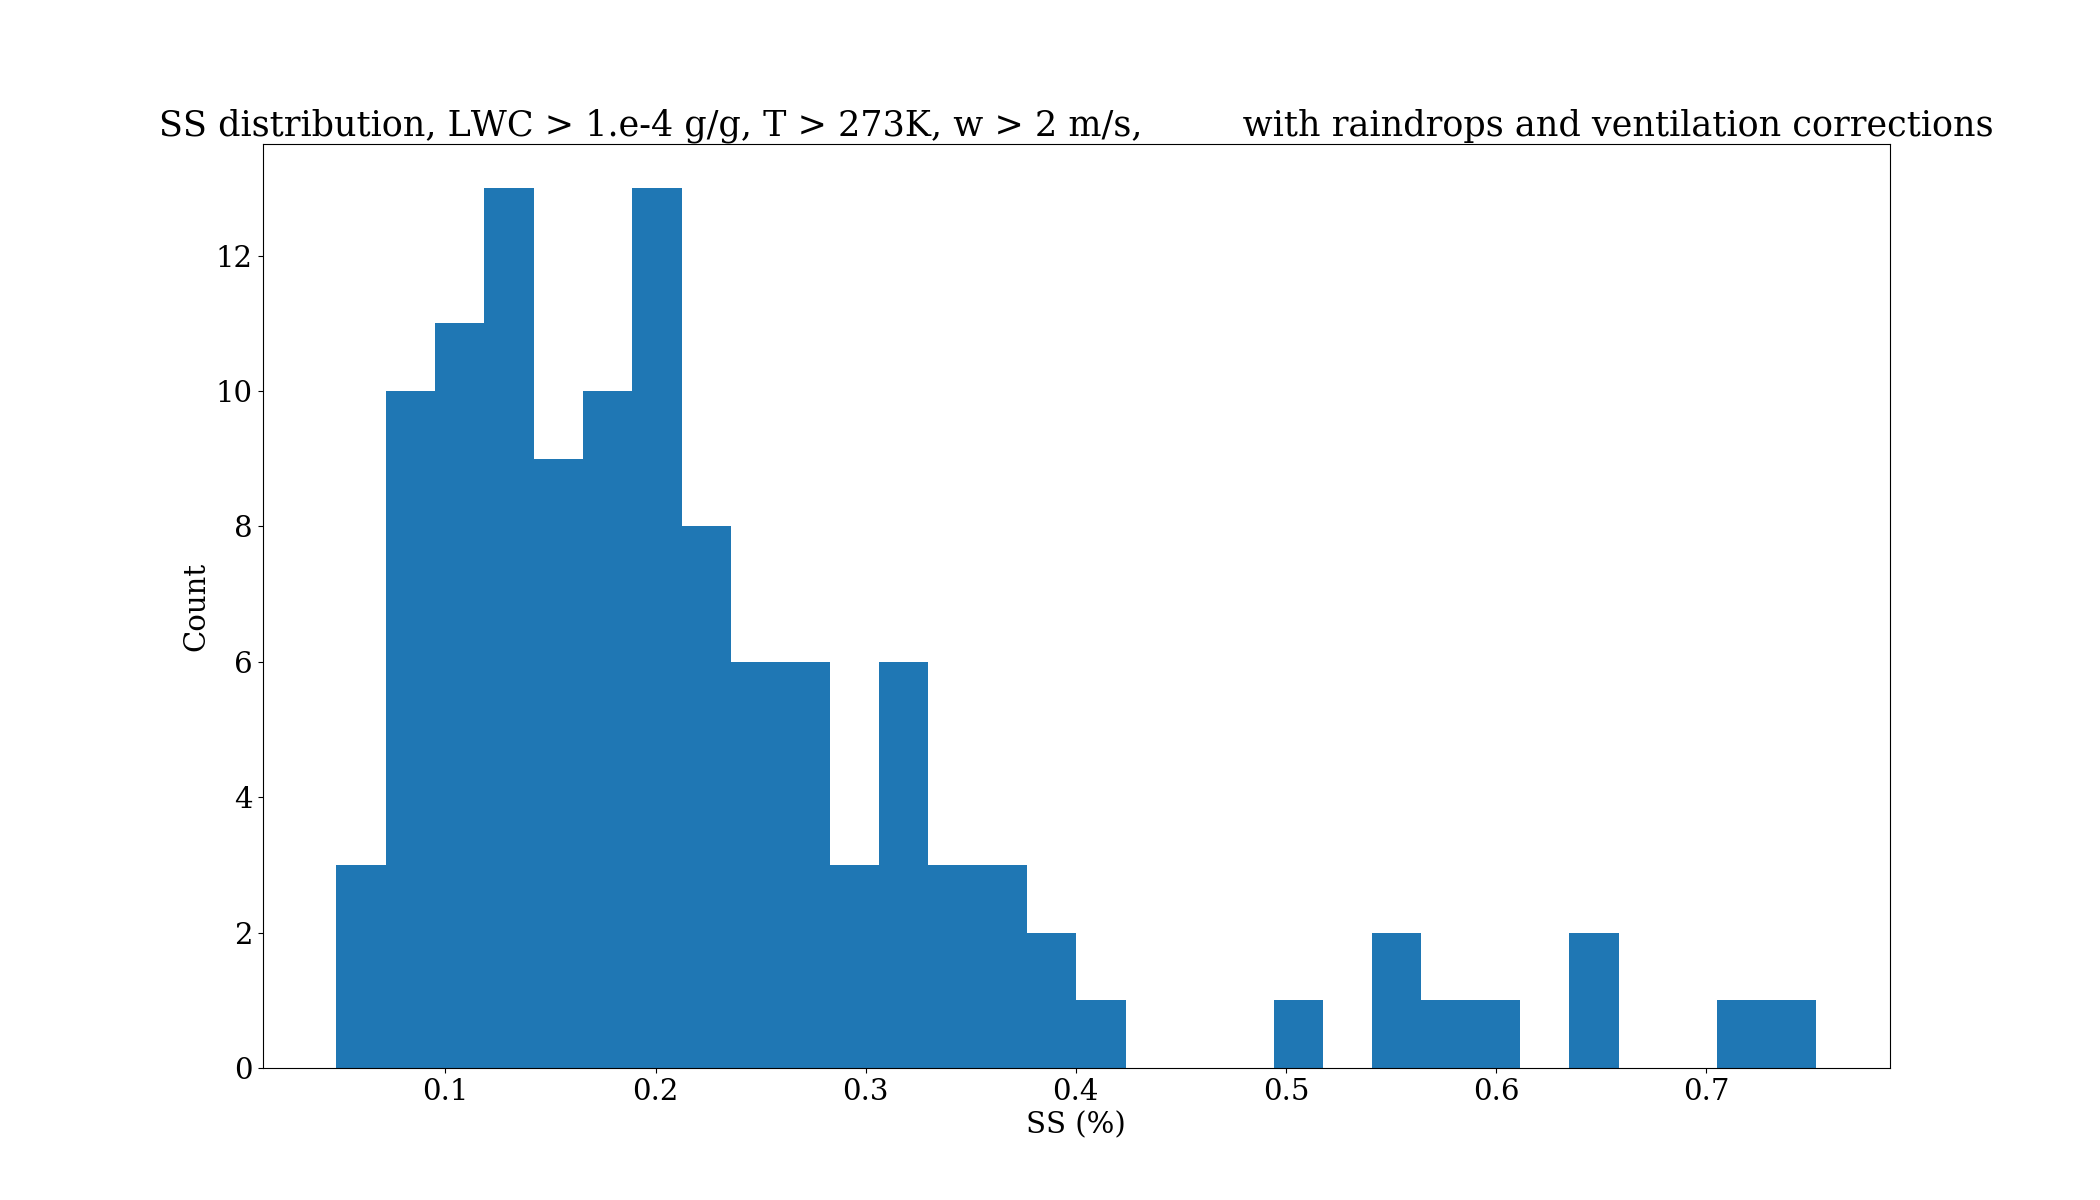
\includegraphics[width=9cm]{halo/v3_ss_with_cip_from_cas_alldates_figure.png}
%    \caption{}
%    \label{fig:fig_label}
%\end{figure}

\bibliography{refs}
\bibliographystyle{ieeetr}
\end{document}
